\documentclass[nobib]{tufte-handout}

%\\geometry{showframe}% for debugging purposes -- displays the margins

\newcommand{\bra}[1]{\left(#1\right)}
\usepackage{clrscode3e}
\usepackage{hyperref}
\usepackage[activate={true,nocompatibility},final,tracking=true,kerning=true,spacing=true,factor=1100,stretch=10,shrink=10]{microtype}
\usepackage{color}

% Fixes captions and images being cut off
\usepackage{marginfix}

\usepackage{tikz}
\usepackage[american currents, american resistors, american voltages]{circuitikz}
\usepackage{amsmath,amsthm}
\usetikzlibrary{shapes}
\usetikzlibrary{positioning}

% Set up the images/graphics package
\usepackage{graphicx}
\setkeys{Gin}{width=\linewidth,totalheight=\textheight,keepaspectratio}
\graphicspath{{.}}

\title{Notes for PHYS 27200 - Electric And Magnetic Interactions}
\author[Ezekiel Ulrich]{Ezekiel Ulrich}
\date{\today}  % if the \date{} command is left out, the current date will be used

% The following package makes prettier tables.  We're all about the bling!
\usepackage{booktabs}

% The units package provides nice, non-stacked fractions and better spacing
% for units.
\usepackage{units}

% The fancyvrb package lets us customize the formatting of verbatim
% environments.  We use a slightly smaller font.
\usepackage{fancyvrb}
\fvset{fontsize=\normalsize}

% Small sections of multiple columns
\usepackage{multicol}

% These commands are used to pretty-print LaTeX commands
\newcommand{\doccmd}[1]{\texttt{\textbackslash#1}}% command name -- adds backslash automatically
\newcommand{\docopt}[1]{\ensuremath{\langle}\textrm{\textit{#1}}\ensuremath{\rangle}}% optional command argument
\newcommand{\docarg}[1]{\textrm{\textit{#1}}}% (required) command argument
\newenvironment{docspec}{\begin{quote}\noindent}{\end{quote}}% command specification environment
\newcommand{\docenv}[1]{\textsf{#1}}% environment name
\newcommand{\docpkg}[1]{\texttt{#1}}% package name
\newcommand{\doccls}[1]{\texttt{#1}}% document class name
\newcommand{\docclsopt}[1]{\texttt{#1}}% document class option name

% Define a custom command for definitions
\newcommand{\defn}[2]{\noindent\textbf{#1}:\ #2}

\begin{document}

\maketitle

\begin{abstract}
These are lecture notes for fall 2023 PHYS 27200 at Purdue. Modify, use, and distribute as you please.
\end{abstract}

\tableofcontents

\section{Course Introduction}

This is a calculus-based physics course using concepts of electric and magnetic fields and an atomic description of
matter to describe polarization, fields produced by charge distributions, potential, electrical circuits,
magnetic forces, induction, and related topics, leading to Maxwell's equations and electromagnetic
radiation and an introduction to waves and interference. 3-D graphical simulations and numerical problem
solving by computer are employed throughout. For more information, consult the syllabus.

\pagebreak 

\section{Equations}

\begin{enumerate}
    \item Coulomb's Law: $\vec{F} = \frac{1}{4\pi \epsilon_0}\frac{q_1 q_2}{r^2}\hat{r}$
    \item Electric field due to a point or charged sphere: $\vec{E_1} = \frac{1}{4\pi \epsilon_0}\frac{q_1}{r^2}\hat{r}$
    \item Force due to electric field: $\vec{F_2} = E_1 q_2$
    \item Dipole moment between charges $-q$ and $q$ separated by $\vec{s}$: $\vec{p} = q\vec{s}$
    \item Electric field on dipole axis: $\frac{1}{4\pi \epsilon_0}\frac{-2sq}{r^3}\hat{p}$
    \item Electric field on dipole bisecting plane: $\frac{-1}{4 \pi \epsilon_0}\frac{sq}{r^3}\hat{p}$
    \item Electric field from point charge-induced dipole: $\left(\frac{1}{4\pi \epsilon_0}\right)^2 \frac{2 \alpha q_1}{r^5}\hat{r}$
    \item Electric field from dipole-induced dipole: $\left(\frac{1}{4\pi \epsilon_0}\right)^2 \frac{12 \alpha p_1^2}{r^7}$
    \item Electric field of a uniformly charged thin rod at a distance $r$ from the midpoint,
    perpindicular to the rod: $\frac{1}{4 \pi \epsilon_0}\left[\frac{Q}{r\sqrt{r^2+(L/2)^2}}\right]$
    \item Electric field due to a charged ring, along the axis of the ring:
    $\frac{1}{4 \pi \epsilon_0}\frac{xQ}{\left(x^{2}+r_{1}^{2}\right)^{\frac{3}{2}}}$
    \item Electric field due to a charged disk, along the axis of the disk:
    $\frac{1}{2 \epsilon_0}\left(\frac{Q}{\pi r_{1}^{2}}\right)x\left(\frac{1}{x}-\frac{1}{\sqrt{r_{1}^{2}+x^{2}}}\right)$
    \item Electric field due to a uniformly charged insulating ball within the ball: 
    $\frac{Q}{4\pi \epsilon_0}\frac{r}{R^3}\hat{r}$
    \item Electric potential in a uniform electric field: $\Delta V = -E\Delta x$
    \item Work and potential: $W = q\Delta V$
    \item Electric potential in a nonuniform electric field: $\Delta V = -\int_{i}^{f} \vec{E} \cdot \vec{l}$
    \item Electric potential of a point charge, at a distance $r$: $\Delta V = \frac{1}{4\pi \epsilon_0}\frac{q}{r}$
    \item Electric field within insulator: $E_{net} = \frac{E_{applied}}{K}$
    \item Potential difference in capacitor with insulator: $\Delta V_{ins} = \frac{\Delta V_{vac}}{K}$
    \item Charge on capacitor: $Q=\frac{\epsilon_0 AKV}{d}$
    \item Energy density of electric field in capacitor: $\frac{U}{\text{volume}} = \frac{1}{2} \epsilon_0 E^2$
    \item Magnetic field at a distance $\vec{r}$ due to a charge $q$ moving at velocity $\vec{v}$: $\vec{B} = \frac{\mu_0}{4 \pi}\frac{q\vec{v}\times \hat{r}}{r^2}$
    \item Magnetic force $\vec{F}$ on charge $q$ moving at velocity $\vec{v}$ in magnetic field $\vec{B}$: 
    $\vec{F} = q\vec{v} \times \vec{B}$
    \item Magnitude of magentic force $F$ on charge $q$ moving at speed $v$ in magnetic field of strength $B$
    with angle $\theta$ between magentic field vector and velocity: $F = qvB\sin(\theta)$
    \item Electron current for $n$ charges per unit volume: $i = nA\bar{v}$
    \item Drift speed: $\bar{v} = uE$
    \item Electric field within wire: $E = \frac{I}{\mu n e A} = \frac{V}{L}$
    \item Magnetic field of a straight wire a distance of $r$ along the bisecting plane: 
    $\frac{\mu}{4 \pi} \frac{IL}{r\sqrt{r^2+(L/2)^2}}\hat{\theta}$
    \item Magnetic field due to an infinite wire: $\frac{\mu_0}{4 \pi} \frac{2I}{r}\hat{\theta}$
    \item Magnetic field due to a loop: $\frac{\mu_0}{4 \pi} \frac{2 \pi R^2 I}{(z^2+R^2)^{3/2}}$
    \item Magnetic field far from a loop: $\frac{\mu_0}{4 \pi}\frac{2 \mu}{z^3}$
    \item Magnetic field due to a coil of length $L$ with $N$ loops: $\frac{\mu_0 nI}{2} \frac{L}{\sqrt{(L/2)^2 + R^2}}$
    \item Current through a loop with height $h$ moving out of a magnetic field $B$ at speed $v$ with resistance $R$: $I = \frac{vBh}{R}$
    \item Force on said loop: $IhB$. 
    \item emf on loop of area $A$ rotating at $\omega$ in magnetic field $B$: $\omega B A \sin(\omega t)$
    \item Approximate magnetic field due to a coil: $\frac{\mu_0 N}{LI}$
    \item Cyclotron frequency: $\omega = \frac{|q|B}{m}$
    \item Magnetic dipole moment: $\mu = IA$
    \item Radius of curvature in magnetic field: $r = \frac{mv}{qB}$
    \item Charge on charging capacitor in an RC circuit: $Q(t) = V_{emf} C (1-e^{-t/RC})$
    \item Charge on discharging capacitor in an RC circuit: $Q(t) = V_{emf} C e^{-t/RC}$
    \item Current through capacitor in an RC circuit: $I(t) = \frac{V_{emf}}{R}e^{-\frac{t}{RC}}$
    \item Equivalent resistance for resistors in series: $R_{eq} = R_1 + R_2 + \dots + R_n$. 
    \item Equivalent resistance for resistors in parallel: $\frac{1}{R_{eq}} =frac{1}{R_1} + \frac{1}{R_2} + \dots + \frac{1}{R_n}$
    \item Equivalent capacitance for capacitors in series: $\frac{1}{C_{eq}} =frac{1}{C_1} + \frac{1}{C_2} + \dots + \frac{1}{C_n}$
    \item Equivalent capacitance for capacitors in parallel: $C_{eq} = C_1 + C_2 + \dots + C_n$
\end{enumerate}

\pagebreak

\pagebreak 

\section{Electric charge}

\defn{Electric Charge}{Electric charge is an intrinsic characteristic of the
fundamental particles that make up objects.}

\marginnote{It was mentioned in class that mass is likewise intrinsic. 
However, when discussing the Higgs field's role in giving particles mass, 
the distinction between mass as an intrinsic or emergent property becomes 
more nuanced. The mass of elementary particles like electrons and quarks is 
emergent in the sense that it arises from their interaction with the Higgs 
field, which itself is a fundamental aspect of the universe.}

\defn{Conservation of charge}{The net charge of a \emph{closed system} never changes}

Objects can have negative, zero, or postive charge. 
Charges are always multiples of the \emph{elementary charge} $e = 1.60217662(63) \times 10^{-19} C$

\defn{Coulomb (C)}{One coulomb is the amount of charge that is
transferred through the cross section of a wire in 1 second
when there is a current of 1 ampere in the wire.}

The charges of elementary particles are listed below.
\begin{table}[ht]
    \centering
    \begin{tabular}{@{}ll@{}}
    \toprule
    Particle & Charge (elementary charge, $e$) \\
    \midrule
    Electron ($e^-$) & $-1$ \\
    Positron ($e^+$) & $+1$ \\
    Proton ($p^+$) & $+1$ \\
    Anti-proton ($p^-$) & $-1$ \\
    Neutron& $0$ \\
    Anti-neutron & $0$ \\
    Photon& $0$ \\
    \bottomrule
    \end{tabular}
    \end{table}

\defn{Point Charge}{A charged object whose
radius is much smaller than the distance
between itself and all other objects of
interest.}

The magnitude of electric force between two point charges is d
irectly proportional to the magnitude of each charge and 
inversely proportional to the distance squared. Specifically:
\[F = \frac{1}{4\pi \epsilon_0}\frac{q_1 q_2}{r^2}\]
This is Coulomb's Law. Note the direction of the force changes
with the sign of the charges involved. Like repels like and opposites
attract. 

\pagebreak 

\section{Electric field}

\begin{marginfigure}
    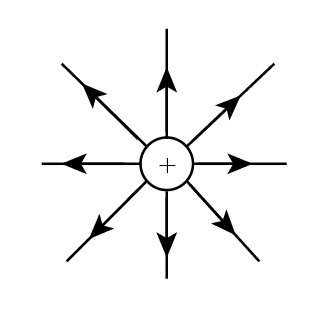
\includegraphics{images/electricfieldlines.jpg}
    \caption{An Electric field coming from point charge. 
    Notice how the densities of the lines vary with distance from the source.}
    \label{fig:electric-field-lines-point-charge}
\end{marginfigure}
Consider a charged particle. We can represent its effect
by drawing vectors that show the path a positively charged 
particle would follow if placed within its influence. These lines represent the 
electric field of the charged particle. The greater the density of the lines, the greater 
the strength of the electric field. Note that at the origin, the force is
undefined (infinite), since $|r| = 0$. 

There are many types of fields, which can be either scalar 
or vector. 
\marginnote{Technically, fields can be the more general tensor,
or even the fascinating and exotic spinor!}
For example, a temperature map is a scalar field, since
each point is associated with a scalar (the temperature at that 
point). A map of fluid velocity is a vector field, since each point 
is associated with a vector (the velocity of the fluid at that point).
For a particle, the Electric field vector at any point is given by
\[\vec{E_1} = \frac{1}{4\pi \epsilon_0}\frac{q_1}{r^2}\hat{r}\]
The direction in which the field lines point depends on the 
sign of the charge. If the charge is negative, the field lines point in.
If it is positive, the field lines point out. A useful mnemonic is
to think of the charge as someone's STD test results. If it's negative,
others will go for them and the lines point in. If it's positive, everyone
will try to get away and the lines point out.

Consider the relative strengths of the electric and 
gravitational fields. The gravitational force is given by
$F_g = G\frac{m_1m_2}{r^2}\hat{r}$, with $m_{electron} = 9 \times 10^{-31} kg$
and $m_{proton} = 1.7 \times 10^{-27} kg$. If we consider a hydrogen atom,  
then $r = 5.3 \times 10^{-11} m$. With $G = 6.7 \times 10^{-11}$, we have 
\[F_g = \frac{(1.7 \times 10^{-27})(9 \times 10^{-31})(6.7 \times 10^{-11})}{(5.3 \times 10^{-11})^2} \approx O(10^{-46})N\]
Now, the Electric force is given by $\vec{F} = \frac{1}{4\pi \epsilon_0}\frac{q_1 q_2}{r^2}\hat{r}$. 
The charge of a proton and Electric are $q_1 \approx q_2 \approx 1.6 \times 10^{-19} C$.
Ergo, since $\frac{1}{4\pi \epsilon_0} \approx 8.99 \times 10^9 \frac{Nm^2}{C^2}$, 
\[F_e = \frac{(8.99 \times 10^9 \frac{Nm^2}{C^2})(1.60\times10^{-19}C)^2}{(5.3\times10^{-11}m)^2} \approx O(10^-17)N\]
This means that $\frac{F_e}{F_g}\approx 2.27 \times 10^{39}$, meaning the Electric force is
much stronger for these masses and charges than gravity. On scales as large as humans and planets,
gravity is the dominant force because gravity is strictly additive.

For sufficient distances, the Electric field
of a uniformly charged spherical shell resembles
the Electric field of a point charge. 

\begin{marginfigure}
    \begin{center}
    \begin{tikzpicture}
        % Dot
        \fill (0,0) circle (1pt);
        % Arrow
        \draw[->] (0,0) -- (0,3);
    \end{tikzpicture}
    \end{center}

    \caption{Notice how a circle resembles a point from a great distance.}
    \label{fig:long-distance-point-sphere}
\end{marginfigure}

That means for $r>>R$, $\vec{E_{sphere}} = \frac{1}{4\pi \epsilon_0}\frac{q_1}{r^2}\hat{r}$
This holds only for outside the sphere. Inside, it can be shown that the electric field is zero. 

\defn{Superposition Principle}{The net electric field at a location in space is a
vector sum of the individual electric fields contributed by all
charged particles located elsewhere.}

To introduce systems with multiple sources of electric field lines, consider
the particle pair known as a dipole. Dipoles consist of one negatively charged
and one positively charged particle, like so:
\begin{marginfigure}
    \centering
    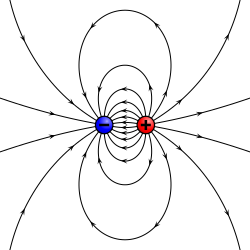
\includegraphics[width=\textwidth / 2]{images/VFPt_dipole_electric.svg.png}
    \caption{Two oppositely charged particles distanced from one another}
    \label{fig:dipole}
\end{marginfigure}

\defn{Dipole Moment}{The dipole moment is a way of expressing asymmetrical charge distribution.
It is a vector quantity, i.e. it has magnitude as well as definite directions.} The
dipole moment is given by the expression $\vec{p} = q\vec{d}$, where $q$ is
the charge on one end of the dipole and $\vec{d}$ is the distance between dipoles.

On the axis of the dipole (i.e. the lines
formed by the two particles), the electric field is 
\[\vec{E} = \frac{1}{4\pi \epsilon_0}\frac{2sq}{r^3}\hat{p}\]
where $r$ is the distance from the point in consideration to the
center of the dipole.
On the bisecting plane (i.e., the plane exactly halfway from each 
point) the field is given by
\[\vec{E} = \frac{-1}{4 \pi \epsilon_0}\frac{sq}{r^3}\hat{p}\]
Where $r$ is the distance from the point to either dipole.
The force on a positive point charge $q_1$ a 
distance of $d$ away from the dipole, aligned with the dipole, and 
on the side of the negative charge is given by 
\[\vec{F}=q_1\vec{E_{dipole}}=q_1(\frac{-1}{4\pi \epsilon_0}\frac{2qs}{d^3},0,0)\]
Note that the field will be parallel to the axis of the dipole: this 
can simplfy vector calculations.
Now consider a dipole in a uniform electric field, like so:
\begin{figure}
    \caption{Dipole in uniform electric field}
    \center
    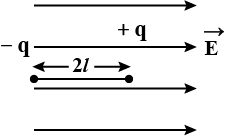
\includegraphics[width=\textwidth /2]{images/dipoleinuniformelectricfield.png}
\end{figure}
The positive end will be pulled to the right and the negative 
end to the left, exerting a torque given by $\vec{\tau} = \vec{p} \times \vec{E_{uniform}}$.
Note that by the definition of $\times$, $\tau = p E_{uniform} \sin{\theta}$, where $\theta$ is the
dipole's angle from horizontal. It can be shown that the potential
energy of a dipole in a uniform Electric field is $U = -\vec{p} \cdot \vec{E_{uniform}}$
and similarly as before (but now with $\cdot$) $U = -p E_{uniform} \cos{\theta}$. Usefully,
this means dipoles can be used to measure the direction of an electric field. 

Throughout these examples, we have been assuming the associated 
speeds are much less than the speed of light. If the velocities
approach a significant fraction of the speed of light Coulomb's
law no longer holds, and we must account for relativity. 

\defn{Conservation of Charge}{Charge cannot be created nor 
destroyed, with the exception of electron-positron annihilation
and other such quantum hijinks.} We can use conservation
of charge to predict the behavior 
\marginnote{Interestingly, in annihilation
between positrons and electrons (or any other 
subatomic particles) the total energy and momentum 
of the initial pair are conserved in the process and 
distributed among a set of other particles in the final state
(photons in the example of the electron-positron pair). 
Antiparticles have exactly opposite additive quantum numbers 
from particles, so the sums of all quantum numbers of 
such an original pair are zero. Hence any set of 
particles may be produced whose total quantum numbers are 
also zero as long as conservation of energy, 
conservation of momentum, and conservation of spin are obeyed.}
of many systems. For example, consider tape pulled from a roll.
You may have noticed when dangling strips of freshly-pulled tape 
they tend to drift towards nearby surfaces to stick and become tangled:
this is because peeling a strip of tape off a roll strips electrons 
from the tape, resulting in a net positive charge because of 
conservation of charge. When this charge approaches a net neutral 
object, such as your hand, the electrons in the atoms of your hand
are attracted to the positively charged tape and congregate closer to the tape.
This results in a negative charge buildup near the tape. The
positive tape is attracted to the negative charges, and so the tape
moves towards your hand and becomes tangled and useless. The process
of one charge inducing a charge on a neutral object occurs 
often enough for the phenomenon to be named. We call it
\defn{Polarization}{The process by which a dipole is formed
in a neutral object by an electric field.} The dipole moment is given by
$\vec{p} = \alpha \vec{E}$, where $\alpha$ is a material-dependent constant
called polarizability. Such a dipole is \emph{induced}. Consider 
a point charge near a neutral atom. The point charge creates an 
electric field given by 
\[\vec{E_1} = \frac{1}{4\pi \epsilon_0}\frac{q_1}{r^2}\hat{r}\]
Inducing a dipole given by the expression
\[\vec{p} = \alpha \vec{E_1} = \frac{1}{4\pi \epsilon_0}\frac{\alpha q_1}{r^2}\hat{r}\]
This dipole creates a field at the point charge of
\begin{align*}
    \vec{E_2} &= \frac{1}{4\pi \epsilon_0}\frac{2\vec{p}}{r^3} \\
    &= \frac{1}{4\pi \epsilon_0}\frac{2\alpha \vec{E_1}}{r^3} \\
    &= \frac{1}{4\pi \epsilon_0}\frac{2\alpha}{r^3}(\frac{1}{4\pi \epsilon_0} \frac{q_1}{r^2}\hat{r}) \\
    &= \left(\frac{1}{4\pi \epsilon_0}\right)^2 \frac{2 \alpha q_1}{r^5}\hat{r}
\end{align*}
This formula is valid provided the electric field that induced the dipole is 
from a point charge. If the electric field is instead from, say, another (permanent)
dipole then $\vec{p} = \alpha \vec{E_1}$ is still valid. However, in this case
the formula for $\vec{E_1}$ will be given by the equation for the electric field
along the axis of a dipole instead. Following this logic, 
\begin{align*}
    \vec{p} &= \alpha \vec{E_1} \\
    &= \alpha \frac{1}{4\pi \epsilon_0}\frac{2\vec{p_1}}{r^3} \\
\end{align*}
If we let $\vec{r'}$ be the location of the permanent dipole from the induced 
dipole, we have the electric field at the permanent dipole as 
\begin{align*}  
    \vec{E}(\vec{r'}) &= \left(\frac{1}{4\pi \epsilon_0}\frac{2}{r^3}\right)\left(\alpha \frac{1}{4\pi \epsilon_0}\frac{2\vec{p_1}}{r'^3}\right) \\
    &= \left(\frac{1}{4\pi \epsilon_0}\right)^2 \frac{4 \alpha \vec{p_1}}{r^3 r'^3}\\
\end{align*}
Calculating the force on the permanent dipole is slightly more complicated than
multiplying by the charge of the dipole, since $r'$ and the sign of 
$q$ varies based on which end of the dipole we consider. To find the net force, we
must find the force on each charge and sum them, like so:
\begin{align*}  
    F^+ &= q\vec{E}(r - \frac{s}{2}) \\
    F^- &= q\vec{E}(r + \frac{s}{2}) \\
    F_{net} &= F^+ + F^- \\
    &= q\left[\left(\frac{1}{4\pi \epsilon_0}\right)^2 \frac{4 \alpha \vec{p_1}}{r^3 (r + \frac{s}{2})^3} - \left(\frac{1}{4\pi \epsilon_0}\right)^2 \frac{4 \alpha \vec{p_1}}{r^3 (r - \frac{s}{2})^3}\right] \\
    &= q\left(\frac{1}{4\pi \epsilon_0}\right)^2 \left[\frac{4 \alpha \vec{p_1}}{r^3 (r + \frac{s}{2})^3} - \frac{4 \alpha \vec{p_1}}{r^3 (r - \frac{s}{2})^3}\right] \\
    &= q\left(\frac{1}{4\pi \epsilon_0}\right)^2\left(4 \alpha \vec{p_1}\right) \left[\frac{1}{r^3 (r + \frac{s}{2})^3} - \frac{1}{r^3 (r - \frac{s}{2})^3}\right] \\
\end{align*}
With a bit more algebraic simplification and the assumption
that $r >> s$, we can show that
\begin{align*}  
    F_{net} &= F^+ + F^- \\
    &= q\left(\frac{1}{4\pi \epsilon_0}\right)^2 \left(\frac{4 \alpha \vec{p_1}}{r^6}\right) \left[(1+\frac{3s}{2r})-(1-\frac{3s}{2r})\right]\\
    &= q\left(\frac{1}{4\pi \epsilon_0}\right)^2 \left(\frac{4 \alpha \vec{p_1}}{r^6}\right) \left[\frac{3s}{r}\right]\\
    &\approx q\left(\frac{1}{4\pi \epsilon_0}\right)^2 \left(\frac{12 \alpha \vec{p_1}s}{r^7}\right) \\
    &= \left(\frac{1}{4\pi \epsilon_0}\right)^2 \frac{12 \alpha p_1^2}{r^7}
\end{align*}

\pagebreak 

\section{Insulators, conductors, and Van der Waals forces}

On the topic of induced dipoles, consider how freely moving
atoms in a substance interact. The electrons are dispersed 
in a cloud about the nucleus of each atom. These clouds can be thought 
of as constantly fluctuating, and occasionally these fluctuations 
will result in more electrons on one side than another. In this 
case there will be a small dipole. If this dipole approaches another
atom (which may or may not have its own temporary dipole) the two will
be attracted. The result of this interaction is that even neutral 
materials can be attracted to each other due to the fluctuating 
dipoles of its electron clouds. We call this phenomenon

\defn{Van der Waals forces}{attraction and repulsions 
between atoms, molecules, as well as other intermolecular 
forces. Caused by correlations in the 
fluctuating polarizations of nearby particles 
(a consequence of quantum dynamics)}.
\begin{marginfigure}
    \caption{Effect of electric field on insulator}
    \center
    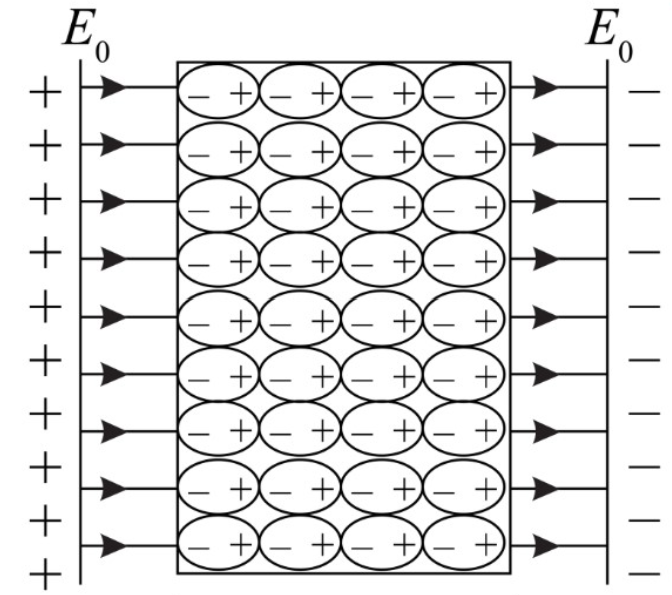
\includegraphics[width=\textwidth/2]{images/insulator.png}
    \label{fig:insulator}
\end{marginfigure}
\defn{Insulator}{An insulator is a material that does not 
easily allow electricity to pass through it}. Inside
an insulator the electrons are bound to their atoms, but they
may still shift in response to an electric field (see fig. \ref{fig:insulator})
This results in the insulator becoming polarized. 
Just as with most polarized objects, we can approximate 
its dipole moment with $\vec{p} = \alpha \vec{E}$
This relationship is only valid if the electrons 
are bound to the stationary constituent atoms. 
If this is not the case, then the a material in 
question is called a

\defn{Conductor}{A conductor is a material 
that allows electricity to flow freely through it}. 
For example, consider a liquid with charged atoms floating
throughout.
\marginnote{Such a liquid is called an \emph{ionic solution}}
Here, when an electric field is applied,
the charges each follow the electric field lines
until they reach the edges of whatever container holds them. 
%show that the electric field within is zero
More commonly, we see conductors in the form of metals. 
The atomic structure of a metal allows electrons to move freely
from atom to atom. Thus, within a metal, the electrons can freely 
move in whichever direction the electric field determines.
\marginnote{Typically electrons are bound to the metal as a whole. However,
if the electric field is strong enough, then air surrounding
a metal can become ionized and allow electrons to flow freely
through it, creating a spark.}
"Freely" is used liberally here, since the electrons 
can collide with other electrons or defects in the metal and lose energy.
The mobile electrons in 
the conductor will have a momentum and velocity given by 
\begin{align*}
    \vec{\Delta p} &= \vec{F_{net}} \Delta t \\
    &= q\vec{E_{net}} \\
    &= -e \vec{E_{net}} \\
    &\rightarrow \vec{\Delta p} = -e \vec{E_{net}} \Delta t \\
    &= m_e v \\
    &\rightarrow v = \frac{e \vec{E_{net}} \Delta t}{m_e}\\
\end{align*}
A good approximation for the average velocity of 
an electron is $\bar{v} = \mu E$. The constant $\mu$ is called
the "mobility". 

Now, consider a conductor with a net charge, such as a charged sphere.
Inside the sphere like charges will repel each another and push 
to get as far away from one another as possible. This occurs when
all the charges are on the surface of the conducting object, since anywhere 
else would be closer together and they cannot go outside the 
bounds of the object. This rearrangement has two effects.
First, any charge in a conductor will be found on the surface.
Second, the net electric field inside a conductor will be zero. 
\marginnote{To see why this must be the case, imagine if it 
were not. Then any charge within the conductor would be moved
by the electric field, so we see that the case where no electric field
is present is the only stable possibility. However, if electrons 
are moving, then there can be (and is) an electric field within
the conductor. It is only when the conductor is in static 
equilibrium that there is no net electric field within.}
An interesting result of electrons seeking to minimize repulsion inside a conductor is 
the \emph{sharp point effect}. To visualize this effect, imagine a gymnasium full of students 
pretending to be electrons, staying as far away from others as possible. 
Anyone near the center of the crowd will feel badly pressed and will try 
to work there way towards the edge of the gym, where at least one side 
will no longer have fellow students milling about. The result? 
Most of the students will gravitate towards the edge of the gym 
and hover there, to take advantage of that lack of other students 
on the wall side of the gym. Now imagine a narrow corridor leading out of the gym. 
Even better! Students in that corridor will only have 
fellow students behind and in front of them.
Now imagine the very end of that corridor, a sort of point. 
Even better! Now, the student who finds that spot will benefit 
from having only one student nearby. But somewhat ironically, 
that same effect will cause other students to pack themselves 
into the long, narrow corridor more tightly, since pretty 
much anywhere in the corridor makes them less exposed to the 
full set of students than being in the gym does.
This effect makes edges, wires, and points more attractive to electrons, 
which similarly just don't want other electrons nearby.

\pagebreak 

\section{Finding electric field}

Now that we understand conceptually how charge behaves in a conductor, 
let's think about the electric field that charge creates. We can
visualize any charged object as a collection of point charges in the shape of 
the object. If we'd like to find the net electric field of these charges, 
we simply use Coulomb's law and sum up each of their electric fields. To 
illustrate this approach, imagine a charged rod with length $L$ and charge $Q$. We can 
approximate it as a bunch of charges in a row. For now, let's use ten, but
recognize that the more charges we use the better our estimate will be. 
Each piece of the rod will have a charge of $\frac{Q}{10}$, so to find 
the electric field at a point we would need to calculate the vector between each piece 
and the point and use $\vec{F} = \frac{1}{4\pi \epsilon_0}\frac{q_1 q_2}{r^2}\hat{r}$. 
We would do this ten times and then sum the electric fields to get our approximate net field. 
Of course, perhaps we would like to find the exact electric field. To do this
we would have to cut our object up into an infinite number of points, find the 
infinitesimal electric field due to each, and sum them up. Sound familiar? 

To drive the point home, consider a vertical rod with a uniform charge of $Q$ and length $L$. 
Let's take a point on the bisecting plane of this rod (the horizontal plane that cuts the rod in half).
Say we view this point from the side and see that is has coordinates $(0, x)$. 
If we want to find the electric field due to a little bit of the rod at $\vec{x}$, 
we need to know the distance between them. If the bit is a distance of $y$ up the rod,
the distance between it and $\vec{x}$ will be $r = \sqrt{x^2 + y^2}$. 
The charge of this small piece will be $\frac{Q}{L} \Delta y$ (where $\Delta y$ is the 
height of the peice), and $\hat{r}$ 
will be $\frac{(x,-y)}{\sqrt{x^2+y^2}}$. 
Therefore the electric field at $\vec{x}$ will be given by 
\begin{align*}
    \Delta \vec{E} &= \frac{1}{4\pi \epsilon_0}\frac{q_1}{r^2}\hat{r} \\
    &= \frac{1}{4\pi \epsilon_0}\frac{\frac{Q}{L} \Delta y}{x^2+y^2}\frac{(x,-y)}{\sqrt{x^2+y^2}}
\end{align*}
We can see by symmetry (isn't symmetry lovely?) that the contributions in the $y$
direction will cancel, so we need only consider the $x$ direction. Therefore, 
\begin{align*}
    \Delta \vec{E} &= \frac{1}{4\pi \epsilon_0}\frac{\frac{Q}{L} \Delta y}{x^2+y^2}\frac{x}{\sqrt{x^2+y^2}} \\
    &= \frac{Q}{4\pi \epsilon_0 L}\frac{x \Delta y}{(x^2+y^2)^{3/2}}
\end{align*}
Now comes the tricky part: adding these up. You have already likely guessed that
we will need to integrate between the bottom and top of the rod, which
corresponds to the integral from $-\frac{L}{2}$ to $\frac{L}{2}$. We have then
\begin{align*}
    \vec{E} &= \int_{-L/2}^{L/2} \frac{Q}{4\pi \epsilon_0 L}\frac{x}{(x^2+y^2)^{3/2}} dy\\
\end{align*}
I'll spare you the tedious integration and skip to the result:
\begin{align*}
    \vec{E} &= \frac{1}{4 \pi \epsilon_0}\left[\frac{Q}{x\sqrt{x^2+(L/2)^2}}\right]\hat{x}\\
\end{align*}
The steps for finding the electric field due to a charged object in general are outlined below.
\begin{enumerate}
    \item Cut up the charge distribution into pieces and draw $\Delta \vec{E}$
    \begin{itemize}
        \item Divide the charge distribution into pieces whose field is known. 
        In particular, very small pieces can be approximated by point particles.
        You may also wish to break up a complex object into smaller objects whose
        electric field equations are already known. 
        \item Pick a representative piece, and at the location of interest draw a 
        vector $\Delta \vec{E}$ showing the contribution to the electric field of this representative piece. 
        Drawing this vector helps you figure out the direction of the net field at the location of interest.
    \end{itemize}
    \item Write an expression for the electric field due to one piece
    \begin{itemize}
        \item Pick an origin for your coordinate system, and show it on your diagram.
        Draw the vector $\vec{r}$ from the source piece to the observation location. 
        Write algebraic expressions for $\vec{r}$ and $\hat{r}$.
        \item Write an algebraic expression for the magnitude $|\Delta \vec{E}|$ contributed by the representative piece. Multiply by
        $\hat{r}$ to get the vector $\Delta \vec{E}$. You can break this up into 
        $x$, $y$, and $z$ components for integration. Once you do each expression should 
        contain one or more “integration variables” ($\Delta x/\Delta y/ \Delta z$ or $dx/dy/dz$) related to the coordinates of the piece.
        Write the amount of charge on the piece, $\Delta q$, in terms of your variables. 
    \end{itemize}
    \item Sum the contributions of all the pieces
    \begin{itemize}
        \item The net field is the sum of the contributions of all the pieces. 
        To write the sum as a definite integral, you must include limits 
        given by the range of the integration variable. If the integral 
        can be done symbolically, do it. If not, choose a finite number 
        of pieces and do the sum with a calculator or a computer.
    \end{itemize}
    \item Check the result
    \begin{itemize}
        \item Check that the direction of the net field is qualitatively correct.
        \item Check the units of your result, which should be newtons per coulomb.
        \item Look at special cases. For example, if the net charge is 
        nonzero, your result should reduce to the field of a point 
        charge when you are very far away. For a numerical integration 
        on a computer, check that the computation gives the correct numerical 
        result for special cases that can be calculated by hand.
    \end{itemize}
\end{enumerate}
Let's apply these steps to some new problems. First, let's consider the electric field
produced by a charged ring (fig. \ref{fig:ring}).
\begin{figure}
    \center
    \caption{Charged ring}
    \label{fig:ring}
    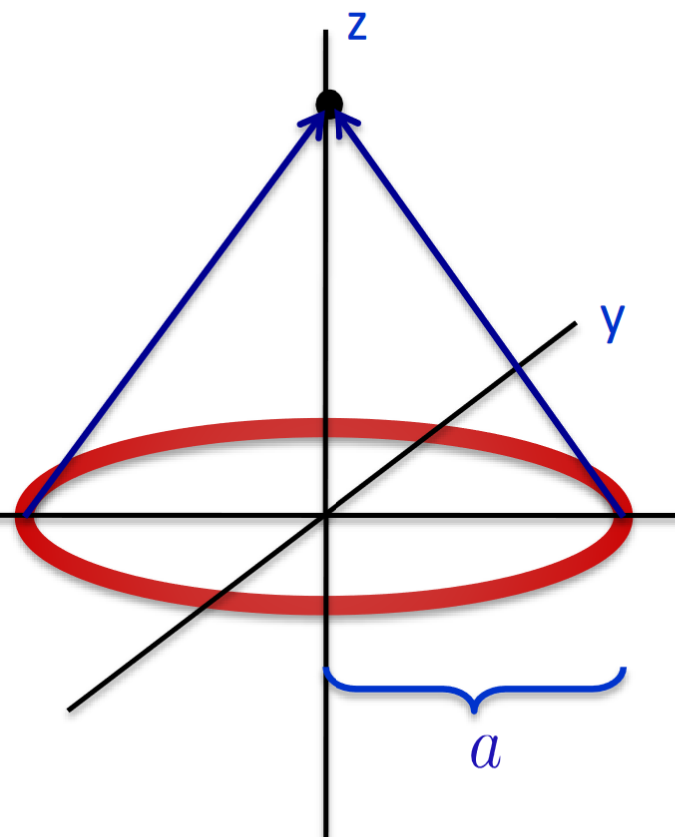
\includegraphics[width=\textwidth/2]{images/ring.png}
\end{figure}
We have a ring of radius $a$, with a charge of $Q$. The ring is centered on the xy plane
and we are calculating the electric field on the z-axis. 
\begin{enumerate}
    \item Cut the charge distribution and find $\Delta \vec{E}$. 
    \begin{figure}
        \center
        \caption{Charged ring slice}
        \label{fig:ringslice}
        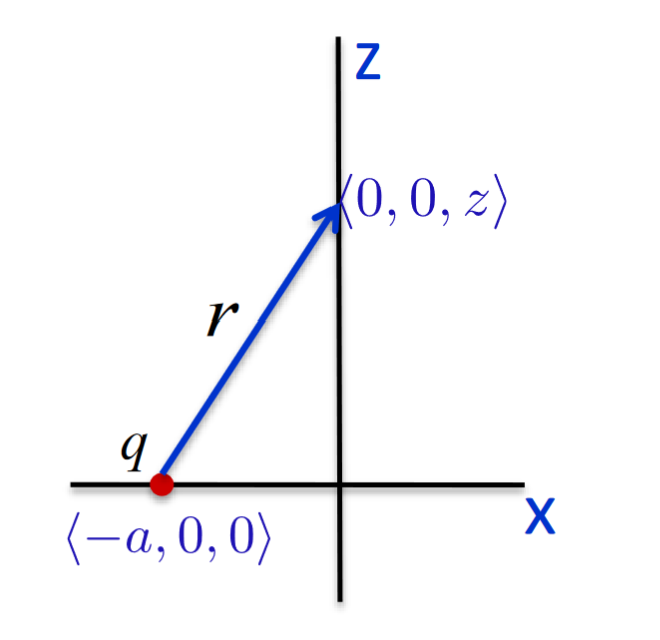
\includegraphics[width=\textwidth/2]{images/ringslice.png}
    \end{figure}
    Let's take a slice of this ring, like fig. \ref{fig:ringslice}. We can 
    view the slice of the annulus here as a point charge a distance 
    of $\sqrt{a^2+z^2}$ away from $(0,0,a)$. We find then that 
    \begin{align*}
        \vec{r} &= (a,0,z) \\
        \hat{r} &= \frac{(a,0,z)}{\sqrt{a^2+z^2}}
    \end{align*}
    %what is \Delta e?
    \item By symmetry, only the z components of each individual electric field
    contribute. Therefore, 
    \begin{align*}
        \vec{E} &= \sum \frac{1}{4 \pi \epsilon_0} \frac{z \Delta q}{(a^2+z^2)^{3/2}}
    \end{align*}
    \item Since the charge is uniformly distributed, we have that 
    $\Delta q = \frac{Q \Delta \theta}{2 \pi}$. 
    Therefore our integral becomes 
    \begin{align*}
        \vec{E} &= \int_0^{2 \pi} \frac{1}{4 \pi \epsilon_0} \frac{z \frac{Q}{2 \pi}}{(a^2+z^2)^{3/2}} d \theta \\
        &= \frac{Q}{4 {\pi}^2 \epsilon_0}\frac{z}{{(a^2+z^2)^{3/2}}} \int_{0}^{2\pi}d\theta \\
        &= \frac{1}{4 \pi \epsilon_0}\frac{Qz}{{(a^2+z^2)^{3/2}}}\hat{z}
    \end{align*}
    \item This looks pretty good. It goes to zero as z goes to either zero or infinity, as it should. 
\end{enumerate}
Let's consider the electric field on the z-axis of a disk with radius $r$ and charge $Q$ now. 
\begin{enumerate}
    \item Take some point on the disk. The calculation for the electric field due to 
    this point is identical to the case of the ring. Therefore 
    \begin{align*}
        \vec{r} &= (a,0,z) \\
        \hat{r} &= \frac{(r,0,z)}{\sqrt{a^2+z^2}}
    \end{align*}
    \item Now we have that $\Delta q = \frac{Q}{\pi r^2} da d\theta$. Therefore
    \begin{align*}
        \vec{E} &= \sum \frac{1}{4 \pi \epsilon_0}\frac{z \Delta q}{(a^2+z^2)^{3/2}} \\
        &= \sum \frac{1}{4 \pi \epsilon_0} \frac{Q}{\pi r^2} \frac{z da d\theta}{(a^2+z^2)^{3/2}}
    \end{align*}
    \item 
    \begin{align*}
        \vec{E} &= \frac{1}{4 \pi \epsilon_0} \frac{Qz}{\pi r^2} \int \int \frac{a}{(a^2+z^2)^{3/2}} da d \theta \\
        &= \frac{1}{4 \pi \epsilon_0} \frac{Qz}{\pi r^2} \int_{0}^{2 \pi} \int_0^{r} \frac{a}{(a^2+z^2)^{3/2}} da d \theta \\
        &= \frac{1}{2 \epsilon_0} \frac{Qz}{\pi r^2} \left[\frac{1}{z} - \frac{1}{\sqrt{r^2 + z^2}}\right] \hat{z}
    \end{align*}
\end{enumerate}
Say we have two conducting disks very near to one another, with opposite charges 
(this configuration is known as a \emph{capacitor}). 
Our equation for the electric field due to a uniformly charged disk does not hold 
for a conductor, since the charges are free to locomote. The charges will be repelled 
to the edges of the disk and attracted to the negative charges in the other disk. 
This attraction means that the charge on the disks will be spread nearly uniformly 
on the inner surfaces of the disks and the field between the plates may be 
approximated as the field between two infinite plates, but what of the outside? 
Some charge will still be on the outer surface of these disks, and his charge will 
create an electric field outside of the capacitor. Not a strong field
in comparison to the inner field, but still nonzero. To calculate it we can use the equation
for electric field due to a uniformly charged disk, 
\begin{align*}
    \vec{E_{disk}} &= \frac{1}{2 \epsilon_0}\left(\frac{Q}{\pi r_{1}^{2}}\right)x\left(\frac{1}{x}-\frac{1}{\sqrt{r_{1}^{2}+x^{2}}}\right) \\
    &\approx \frac{1}{2 \epsilon_0}\frac{Q}{\pi R^2}\left[1-\frac{x}{2R}\right]
\end{align*}
The net field will be the sum of the fields from each disk. Ergo, 
\begin{align*}
    \vec{E} &= \vec{E}_{1} + \vec{E}_{2} \\
    &\approx \frac{1}{2 \epsilon_0}\frac{Q}{\pi R^2}\left[1-\frac{x}{R}\right] + \frac{1}{2 \epsilon_0}\frac{Q}{\pi R^2}\left[1-\frac{s-x}{R}\right] \\
    &\approx -\frac{1}{2 \epsilon_0}\frac{Qs}{\pi R^3}
\end{align*}
With that brief divagation out of the way, let us return our attention to charged spheres. 
Recall that the electric field outside of a charged sphere is given by 
\[\vec{E} = \frac{1}{4 \pi \epsilon_0}\frac{Q}{r^2}\hat{r}\]
provided $r > R$. If we have $r < R$, then we know there is no net electric field within the 
sphere. 
\marginnote{For a very loose explanation of why there is no electric field within a sphere, 
consider the field due to each
bit of the sphere on a point inside. At any point you have some charges nearby and some 
far away, and if that were all to there story then the Electric field would 
point towards the center of the shell. However, you have more charges far away than close.
It works out that the effect of this greater number of charges exactly cancels out the farther
distance and there is no net field within the shell! This is an interesting proof if you care
to work it out.}
Imagine placing a proton inside a charged sphere, and now consider what the field inside will be.
The answer depends on if the sphere is made of a conducting materal or not. If charges are free
to move in the sphere, then they will migrate and exactly cancel out the electric field of 
the proton, since the electric field within a conductor is zero. If the sphere is instead 
made of an insulator, then the electric field inside due to the sphere will still be zero, 
but the proton will now contribute an Electric field of its own according to Coulomb's law. 
What if we have another, concentric insulating charged sphere within the first? Well, if we 
are within both, then the Electric field will still be zero due to the superposition 
principle. If we are outside the bounds of the first but still within the second, then the inner
sphere will have an electric field given by Coulomb's law, while the outer shell still contributes no 
net field. If we are outside both then it appears to use that there is a point with a charge 
that is the sum of the charges of each sphere, and the electric field will again be given by Coulomb's law. 
Well and good, but what if we have a insulating ball, a filled sphere? What is the electric field then?
We know that it will be given by Coulomb's law outside of the ball, but on the inside 
it isn't zero anymore. A=If you picture the ball as a series of concentric shells then the 
shells radially past the inner point will contribute nothing, but you will still have a 
small sphere of charge radially inward with a net field. Let's find the field contributed by this sphere. 
First, cut up the charge distribution and find $\vec{E}$. 
The charge per volume will be 
\begin{align*}
    \frac{Q}{V} &= \frac{Q}{4/3 \pi R^3}
\end{align*}
For a point a distance of $r$ within the ball, we have 
\begin{align*}
    \frac{\Delta q}{4/3 \pi r^3} 
\end{align*}
We know that the sphere is uniformly charged. That is, the charge density everywhere is the same. 
Thus, 
\begin{align*}
    \frac{\Delta q}{4/3 \pi r^3} &= \frac{Q}{4/3 \pi R^3} \\
    \rightarrow \Delta q &= Q\frac{r^3}{R^3}
\end{align*}
So we now have that 
\begin{align*}
    \vec{E} &= \frac{1}{4 \pi \epsilon_0} \frac{Q\frac{r^3}{R^3}}{r^2} \\
    &= \frac{Q}{4\pi \epsilon_0}\frac{r}{R^3}\hat{r}
\end{align*}
And we are done. 

\pagebreak 

\section{Electric potential} 
To begin this section, let's imagine what happens when we touch two 
conductors together. Say one has a charge of 6 nc and the other of 0 nC, 
but otherwise they are identical. What happens when the conductors are brought 
in contact? We intuit that the charge flows from one to the other 
until each has a charge of 3 nC, and this is indeed what would happen. 
Consider a similar situation, but now the conductor of 6 nC is 
much smaller than the neutral conductor. What happens when these two 
are brought in contact now?

As you ponder that, let's briefly review energy. The energy of 
a particle moved by a force $\vec{F}$ along a path $\vec{l}$ is given by 
\[\Delta E_{particle} = W = \int \vec{F} \dot d\vec{l}\]
If the forces involved are conservative, we also have that 
\[\Delta U = -W_{internal}\]
Consider a particle between two charged infinite plates. Let's find the change in its potential energy
as it moves from point A to point B. If the electric field strength is $E$ N/C, 
then 
\begin{align*}
    \Delta U &= -W_{internal} \\
    &= -\int qE d\vec{r} \\
    &= -q\int dx \\
    &= -qE\Delta x \\
    &= -qV
\end{align*}
So the difference in potential energy of a particle inside a charged 
electric field is proportional to the strength of the field and the distance
moved. We can classify the ability to have potential energy 
if a charge enters a system as the

\defn{Electric potential}{the amount of work energy needed 
per unit of electric charge to move this charge from a 
reference point to the specific point in an electric field}.
Mathematically, the potential $\Delta V$ can be expressed as
\[\Delta V = -E\Delta x\]
\marginnote{The astute reader will notice 
that this equation is not very general, 
as it only applies when the charge moves 
in a straight line through a uniform 
electric field. In general, 
\[\Delta V = -\int_{i}^{f} \vec{E} d\vec{l}\]
This integral is a \emph{line integral}. It can be 
computed using multivariable calculus, but sometimes 
it simplifies to a form that makes this approach unecessary.}
V may seem like an odd choice of variable here, but electric 
potential is such an important concept that it gets its own
units of Volts (which are equivalent to J/C).
Despite the fancy name, we can think of electric potential the 
same way as gravitational or any other potential. Charges
will move from high to low potential, just like a ball rolling 
down a hill is moving from high to low potential. 
Here the strength of the electric field is analogous 
to the height of the hill, and the charge is the ball. 
Just as with a hill and a ball, we also need two things 
in order to find electric potential energy. 
\marginnote{What's the potential energy 
of something floating around by itself in space? The question
seems to make no sense, since potential energy is defined as a difference 
between two states. However, the potential at a single point is often defined as the 
potential relative to infinity, $V_A = V_A - V_{\infty}$. The electric potential 
is a scalar field, and has a value at every point in space. }
In the simplest case, 
imagine two charges near one another. The force 
of one on the other is simply 
\[\vec{F} = \frac{q_1 q_2}{4 \pi \epsilon_0 r^2}\hat{r}\]
and as we have learned, 
\[W = \int_{a}^{b}\vec{F} d\vec{x}.\]
So to find the work done as one 
particle goes from A to B, we have 
\begin{align*}
    W &= \int_{a}^{b} \vec{F}dr \\
    &= \int_{a}^{b} \frac{q_1 q_2}{4 \pi \epsilon_0 r^2}\hat{r} dr \\
    &= \frac{q_1 q_2}{4 \pi \epsilon_0} \int_{a}^{b} \frac{dr}{r} \\
    &= \frac{q_1 q_2}{4 \pi \epsilon_0} \left(\frac{-1}{r}\right) \\
    &= \frac{q_1 q_2}{4 \pi \epsilon_0} \left(\frac{1}{a}-\frac{1}{b}\right)
\end{align*}
We can define the \emph{electric potential energy}
of a system of charges as
the work needed to assemble the
system by bringing each
charge from infinity to its
final position. 
\marginnote{\emph{Electric potential energy} is NOT \emph{electric potential}. 
Electric potential energy has a dependency upon the charge of the 
object experiencing the electric field, electric potential is 
purely location dependent. Electric potential is the electric potential 
energy per charge.}
In this case, 
\[U = \frac{q_1 q_2}{4 \pi \epsilon_0 r},\]
where $r$ is the distance between one charge 
and another. For a system with multiple particles, 
the total energy will simply be the sum 
of the energies of each individual charge with 
respect to each other.

Let's calculate the electric potential of three point charges $A,B$, and $C$.
The distances are $r_{12}$, $r_{13}$, and $r_{23}$. The electric potential energy is 
the sum of the individual potential energies. That is, 
\begin{align*}
    U &= \sum U_i \\
    &= \frac{1}{4\pi \epsilon_0}\frac{q_1 q_2}{r_{12}} + \frac{1}{4\pi \epsilon_0}\frac{q_1 q_3}{r_{13}} + \frac{1}{4\pi \epsilon_0}\frac{q_2 q_3}{r_{23}}
\end{align*}

Now, you have probably noticed that, in general, things love moving from high potential to 
low potential. Lift something high up in the gravitational field, and it gains potential, let it go
and it falls and loses potential. Gifted students and especially electric fields follow the same 
principle. The electric field points from the highest potential to the lowest potential, 
dictating how a charge will move if placed in a field. We can see this mathematically, 
since we know 
\begin{align*}
    \Delta V &= -\int_{i}^{f} \vec{E} \cdot d\vec{l} \\
    &\rightarrow dV = -\vec{E}\cdot d\vec{l}
\end{align*}
Since $\vec{l}$ can be multidimensional, to find $dV$ we'd need multivariable calculus. 
If we calculate the derivative what we would get is 
\begin{align*}
    dV &= -\vec{E}\cdot d\vec{l} \\
    &\rightarrow \frac{dV}{d\vec{l}} = -\vec{E} \\
    &= V\left( \frac{\partial}{\partial x} + \frac{\partial}{\partial y} + \frac{\partial}{\partial z} \right) \\
    &= -\nabla V
\end{align*}
If you are familiar with gradients ($\nabla$) you will know this means
the electric field points in the direction in which the potential decreases most rapidly. 
We also know the electric field always points in the direction of
steepest descent of $V$ and its
magnitude is the slope. And just as with gravity, it can be shown that the 
electric potential between two points does not
depend on the integration path. Any path will do. Moreover, any closed path 
has an electric potential of 0. 
\marginnote{Take a momement to convince yourself of this by whatever 
means you find most useful. It can be shown both mathematically 
and intuitively.}
In general, if you know electric field, you may integrate to find 
the electric potential between two points. If you know the potential, 
differentiate. 

If you have a shape, there are two ways to get the potential. 
\begin{enumerate}
    \item Break the object into point changes and add up the potential from each. 
    \item If you know the electric field, use $\Delta V = \int_{a}^{b} E \cdot dl$
\end{enumerate}
Say we have a ring with radius $R$ and charge $Q$. Using method 1, the potential due 
to each charge on the axis is $\Delta V_i = \frac{1}{4\pi \epsilon_0}\frac{\Delta q_i}{r}$.
If we are a distance of $z$ along the axis, $r = \sqrt{z^2+R^2}$, and we have 
\[V = \sum \frac{1}{4 \pi \epsilon_0}\frac{\Delta q_i}{\sqrt{z^2+R^2}}\]
\begin{align*}
    V &= \sum \frac{1}{4 \pi \epsilon_0}\frac{\Delta q_i}{\sqrt{z^2+R^2}} \\
    &= \frac{1}{4 \pi \epsilon_0}\frac{1}{\sqrt{z^2+R^2}} \sum \Delta q_i \\
    &= \frac{1}{4 \pi \epsilon_0}\frac{Q}{\sqrt{z^2+R^2}}
\end{align*}
Let's try to find the potential again, this time using method 2. 
We recall that 
\[\vec{E} = \frac{1}{4 \pi \epsilon_0}\frac{Qz}{(R^2+z^2)^{3/2}}\]
So the potential will be 
\begin{align*}
    V &= -\int_{\infty}^{z} \frac{1}{4 \pi \epsilon_0}\frac{Qz}{(R^2+z^2)^{3/2}} dz \\
    &= - \frac{Q}{4 \pi \epsilon_0}\int_{\infty}^{z}\frac{z}{(R^2+z^2)^{3/2}} dz \\
    &= \frac{1}{4 \pi \epsilon_0}\frac{Q}{\sqrt{z^2+R^2}}
\end{align*}
Identical to the expression previously obtained, as it should be.

Allow me to now briefly remind the reader of 
the relationship between voltage and electric field. 
\[\Delta V = -\int_{i}^{f} \vec{E}\cdot d\vec{l}\]
\[\vec{E} = - \left[ \left(\frac{\partial}{\partial x}V\right)\hat{x} + \left(\frac{\partial}{\partial y}V\right)\hat{y} + \left(\frac{\partial}{\partial y}V\right)\hat{y} \right]\]
If you remember, a conductor inside a capacitor
has no net electric field within its bounds. 
That means the electric field perpindicular to 
the surface is $\frac{\sigma}{\epsilon_0}$, while parallel 
to the surface the electric field is 0. 
That means that $V_f - V_i = 0$ on 
the surface, since any path on the surface has 
no electric field. We say that the surface of 
a conductor is \emph{equipotential}; that is, 
every point has the same voltage. Of course, this 
is only true if the conductor is at equilibrium.
We have no guarantee of charge distribution is the 
conductor is not in electrostatic equilibrium. 
The situation changes if we instead have an insulator 
between the two plates of a capacitor. The electric field 
within an insulator is not zero. The nonzero 
electric field induces dipoles within the molecules 
of the insulator, which then have an electric field of their own. 
It turns out that inside an insulator, the electric field is 
proportional to the applied electric field by a factor of $1/K$, 
where $K$ is called the dielectric constant and is known for various materials. 
Let's see if we can calculate the potential between plates with an insulator between 
them. The problem: a capacitor with a 3mm gap has a potential
difference of 6V. A disk of glass 1mm thick, with
area the same as the metal plates has a dielectric
constant of 2.5. The glass is inserted in the middle
of the gap between the plates. What is now the
potential difference between the plates? 
We know that without the insulator between the plates, the electric 
field will be. 
\begin{align*}
    E &= \frac{\Delta V}{\Delta x} \\
    &= \frac{6V}{0.003 m} \\
    &= 200 \frac{V}{m}
\end{align*}
Inside the glass, 
\begin{align*}
    E_{net} &= \frac{E}{K_glass} \\
    &= \frac{2000}{2.5} \\
    &= 800 \frac{V}{m}
\end{align*}
The total voltage will be the sum of the voltage 
between the first plate and the glass, the two sides of 
the glass, and the glass and the second plate. 
\begin{align*}
    \Delta V &= V_1 + V_2 + V_3 \\
    &= 2000(0.001) + 800(0.001) + 2000(0.001) \\
    &= 4.8 V
\end{align*}
And we are done. 

Since the electric field can perform work, it must have
energy associated with it. The energy depends on the electric field. 
Say you have two plates of charge $Q$ a distance $s$ apart, but instead of 
holding them there, you let one plate go to see how much energy 
you can get out of this setup. You know the force on one plate is 
\[F = \frac{\sigma Q}{2 \epsilon_0}.\]
Additionally, we recall that 
\[Q = \int F dr.\]
Combining these two equations and noticing the bounds on the integral 
will be the distance between the plates, we have 
\begin{align*}
    W &= \int_{0}^{s} \frac{\sigma Q}{2 \epsilon_0} dr \\
    &= \frac{Q\sigma s}{2 \epsilon_0} \\
    &= \frac{Q^2 s}{2 \epsilon_0 A} \\
    &= \frac{1}{2} \epsilon_0 E^2 s A
    &= -U
\end{align*}
We can define the energy density as the potential energy per 
volume. In this case, 
\[\frac{U}{s A} = \frac{1}{2} E^2 \epsilon_0 E^2\]
and for a general electric field, 
\[\frac{U}{\text{volume}} = \frac{1}{2} E^2 \epsilon_0 E^2\]

\pagebreak 

\section{Magnetism}
Electricity and magentism are fundementally intertwined in many ways. 
A moving electrically charged particle creates a magentic field.
\marginnote{Note that this magentic field is different than the particle's electric field. 
}
Here is some information about magnetism: 
\begin{itemize}
    \item The needle of a compass aligns 
    with the direction of the net magnetic field at its location.
    \item An electric current is a continous flow of charge.
    \item The superposition principle is still valid for 
    magentic fields, so to calculate the net magnetic field we can 
    simply sum individual magentic fields. 
    \item The units of magentic field are Teslas ($T$) or Gausses ($G$). 
    $1 G = 10^{-4} T$. 
    \item Magentic fields are typically symbolized by the letter $B$. 
    \item The earth has a magentic field approximately $.5 G$ strong.  
\end{itemize}
\marginnote{This was confirmed in 1820 when a Danish physicist, Hans Christian Oersted, 
discovered if you held a compass near a live wire the needle deflected.  
Thus Oersted showed that moving electrons can create a magnetic field.
}
You have likely seen and played with magnets before, 
and already know some of their properties. You know that similar poles 
repel one another, and like poles attract. You know magents attract ferromagnetic 
materials (like iron, cobalt, or nickel).  
A magnet is any material or object that produces a magnetic field. 
A type of magnet you are likely familiar with 
is the bar magnet, which looks like fig. \ref{fig:bar}.
\begin{figure}
    \center
    \caption{Bar magnet}
    \label{fig:bar}
    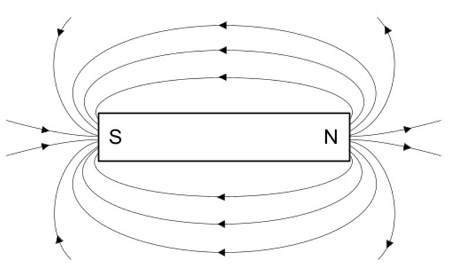
\includegraphics[width=\textwidth/2]{images/bar_magnet.jpg}
\end{figure}
The lines emanating from the north pole and entering the south 
are magentic field lines.  

I have previously said that a moving electric charge produces a magnetic field. 
The equation for the field a distance $\vec{r}$ from a charge $q$ moving at velocity $\vec{v}$ is given by the following law,
called the Biot-Savart law:
\marginnote{$\mu_0$ is a constant, defined to be $4 \pi \times 10^{-7}$. So 
$\frac{\mu_0}{4 \pi} = 10^{-7}$}
\marginnote{Recall that the magnitude of the cross product of two vectors $A$ and 
$B$ at an angle $\theta$ from one another is defined as 
\[A \times B = |A||B|\sin{\theta}.\]
The full cross product can be found using the following formula: 
\[A \times B = (a_2b_3-a_3b_2)\hat{i} + (a_1b_3-a_3b_1)\hat{j} + (a_1b_2-a_2b_1)\hat{k}\]
assuming $a_i$ is the $i$th component of $A$ and likewise for $B$. 
}
\[\vec{B} = \frac{\mu_0}{4 \pi}\frac{q\vec{v}\times \hat{r}}{r^2}\]
Since current is just a bunch of moving charges flowing through a wire, 
then we should expect a current-carrying wire to have a magnetic field, 
and it does. 
The magnetic field looks like fig. \ref{fig:wire}. 
\begin{figure}
    \caption{Magentic field of live wire}
    \label{fig:wire}
    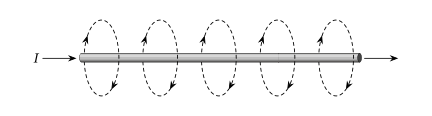
\includegraphics{images/wire.png}
\end{figure}
It is given by the equation
\[B = \frac{\mu_0 I}{2\pi r}\]
If you have calculated the magnitude of the magentic field and wish 
to find its direction, there is another right-hand-rule to follow, 
not to be confused with the right-hand-rule that allows one to find 
the direction of magentic field for a moving charge. 
Point your thumb along the direction of conventional current 
in the wire. Your fingers will curl in the direction of the magentic 
field. 

Although we now know that the mobile charges in a wire are electrons, 
current is conventionally definded as following from flowing from 
the positive to negative terminal of a battery (that is, positive charges 
moving). 
\begin{marginfigure}
    \center 
    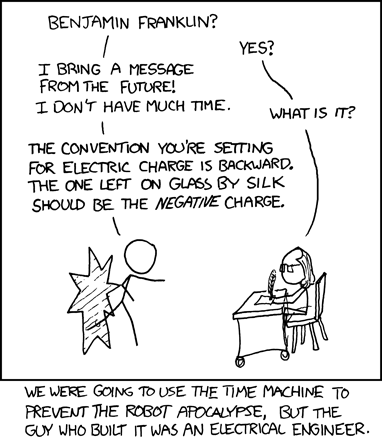
\includegraphics{images/urgent_mission.png}
\end{marginfigure}
\noindent Despite this, we sometimes want to find the \emph{electron current}, 
the number of electrons that flow through a given volume per second. 
Mathematically, the electron current $i$ is given by  
\[i = nA\bar{v},\]
where $n$ is $\frac{electrons}{m^3}$, $A$ is cross sectional area of the wire, and
$\bar{v}$ is the average velocity of electrons in the wire. 
Electron current is what's physically happening, but since we're stuck 
with convention, let's try to think in conventional current. 
Electron current flowing one way is equivalent to conventional current 
flowing the other way. 

So far, we have only examined magnetic fields due to moving charges. 
How can we explain the magnetic field of permanent magnets? What charge 
moves in a stationary object? The answer is the electrons. Within the 
magnet, electrons are moving about their nuclei and spinning on an axis. 
Both of these movements contribute to create a magnetic dipole.
If the magnetic fields 
from other electrons don't cancel out, then there will 
be a net magnetic field on the atom! In order for the magnetic fields of the 
electrons to not cancel, the atom must half a half-full outer shell. When 
the atomic magnetic dipole moments align, the material is known as a ferromagnet
and will have a net magnetic field. 
\marginnote{The magnetic field of permanent magnets can be destroyed by heating the magnet. 
The temperature below which atomic magnets align
is called the "Curie Temperature," and is a phase
transition of the electrons inside a material! In the 
case of iron, it's approximately $1000 K^{\circ}$}
Eletron magnetic dipole is a fundementally quantum mechanical phenomenon,
but in class we treat atoms like a classical system,
where the electron orbits in a loop around the nucleus. From this 
we derive the equation for magnetic dipole of an atom as
\[\mu = \frac{1}{2} eRv.\]
\marginnote{To treat it properly as a quantum system, 
we would need to solve the Schrodinger wave equation
for a hydrogen atom. This is a bit above our pay grade, 
but it turns out that the classical approximation is not bad.}
For our purposes, there are three kinds of magnetism
\begin{enumerate}
    \item Ferrmagnetism, the permanent magnetism explained by the 
    magnetic moments of atoms within the material. 
    \item Paramagnetism, the kind of magnetism that occurs when 
    the magnetic moments in a material only align in response 
    to an external magnetic field. This is why certain metals can be 
    picked up despite having no magnetic field of their own. 
    \item Diamagnetism, where the magnetic moments in the material align 
    opposite to the applied magentic field. This causes diamagnetic objects 
    to be repelled by a magnetic field. 
\end{enumerate}

\section{Circuits}
A \emph{circuit} is a complete circular path that electricity flows through.
Usually, the current is flowing through a wire. There are three states a circuit 
can be in. 
\begin{enumerate}
    \item Equilibrium: no current flows. The average drift velocity of the electrons is 0. 
    \item Transient: when the current is changing, usually after elements are hooked up. 
    \item Steady-state: current is flowing. The average drift velocity is nonzero, 
    and there is no change in the deposits of excess charge on the wire anywhere.
\end{enumerate} 
Equilibrium is rather boring, so let's focus on transient and steady-state. Imagine connecting 
a battery to a loop of wire. Just after the circuit is connected, the circuit is in transience.
There is a disturbance in the previous (equilibrium) electric field right next to the battery. 
At the speed of light, the region next to the disturbance updates its electric field in response, 
and the next region updates, and so on until steady state is achieved.

Importantly, when a circuit is in steady-state, the current at the start equals the current 
at the end. 
Since current is just the flow of electrons, the current needs to be conserved
in the same way charge is conserved. I.e. current in is current out, current can't be "used up",
so on. You may wonder how a current lights a lightbulb if it isn't used up - wouldn't that violate 
conservation of energy? The answer is no, whatever is driving the current powers the lightbulb. Think 
of it like water flowing and turning a turbine that lights the bulb. Water in is water out, but the energy
comes from whatever propelled the water through. In the case of water and a turbine the energy comes from 
kinetic energy and is transferred to electric energy, in the case of the lightbulb the energy usually 
comes from stored potential in a battery. As the electrons collide with the atoms in the bulb filament, 
light and heat are produced. In order to keep shoving these electrons along there needs to be an electric 
field within the wire. This field is produced by an uneven distribution of charge on the wire: electrons 
piled up at one terminal repel other electrons to the other terminal, like in figs. \ref{fig:ringsofpower}
and \ref{fig:chargedistr}
\begin{figure}
    \center
    \caption{Electric field in circuit}
    \label{fig:ringsofpower}
    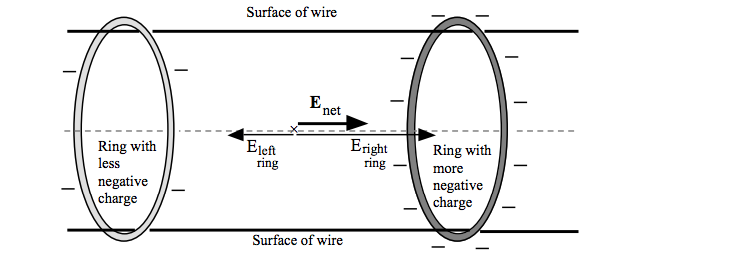
\includegraphics{images/bfucc.png}
\end{figure}
\begin{figure}
    \center
    \caption{Charge distribution in a wire}
    \label{fig:chargedistr}
    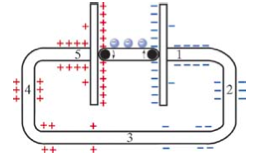
\includegraphics{images/L5thM.png}
\end{figure}
This means that in a circuit, there is a pile of negative charge where the electrons are coming out,
and a pile of positive charge at the other end. 

The analogy of water continues to be useful when you consider a wire with variable 
cross-sectional area. Just as water rushing through a pipe picks up speed when the pipe 
narrows (think of putting your thumb over the end of a hose), the drift velocity
increases when the wire narrows. 
\marginnote{Note that the current is still constant provided the circuit is 
in steady-state, although the drift velocity can change.}
The electric field and drift velocity both increase in order to keep 
the current constant, according to the equation 
\[I = |q|nAu|E|\]
where $|q|$ is the charge on an electron, $n$ is the number of electrons per 
volume of material, $A$ is the cross-sectional area in consideration, 
$u$ is the electron mobility (a constant that determines how quickly 
an electron can move through a material), and $E$ is the strength of the electric field
at that point. The electric field at every point in the wire is actually parallel 
to the wire at that point (see fig. \ref{fig:efww})
\begin{figure}
    \center
    \caption{Electric field within a wire}
    \label{fig:efww}
    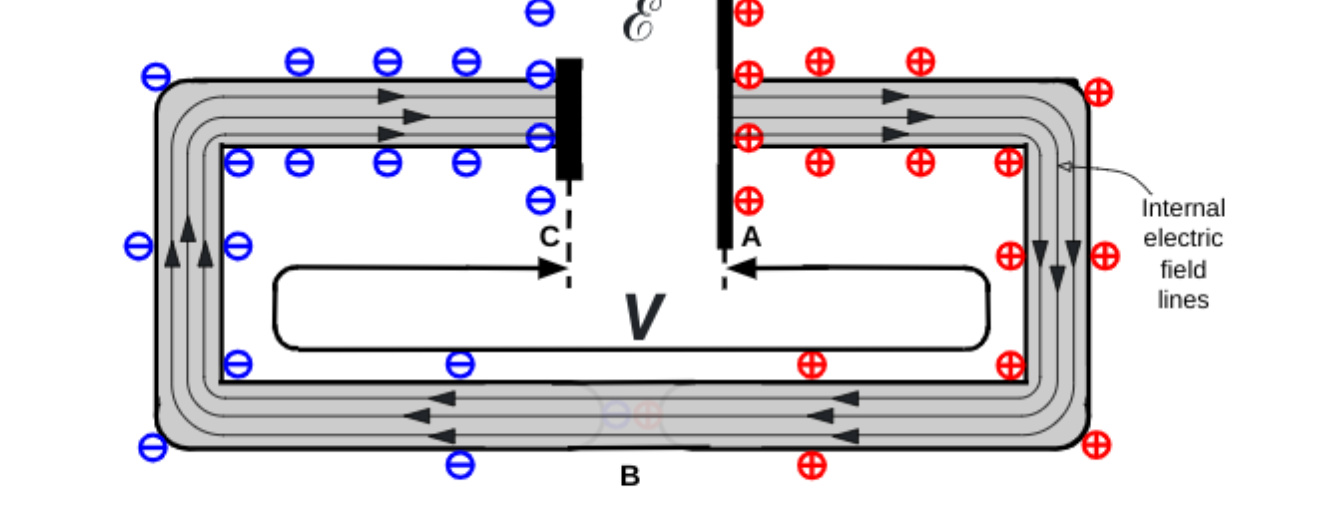
\includegraphics{images/eflineswire.png}
\end{figure}

We usually make the assumption that wires
are ideal and allow current to flow 
freely. Elements for which this is not 
the case are called \emph{resistors}. 

\defn{Resistor}{a part of the circuit that resists 
the passage of electrons.}
Placing a resistor in a circuit reduces 
the overall electric field of the circuit, 
but within the resistor, the electric field is higher 
in order to force eletrons along and maintain a 
constant current. 

Now, as you are familiar with voltage and the general
concept of potential, this next part should be no surprise to you.
We are now going to discuss \emph{Kirchhoff's loop rule}. 
The rule states that the total change in eletric potential 
as you move around a circuit is zero. That is sensible, 
since no matter where you go in an eletric field, if you return 
to the same point you will have the same potential 
regardless of what you did between leaving and coming back. 
\marginnote{This is analogous to gravitational potential and height. 
If you climb a tree, then jump down, then run in circles, 
and climb back up the tree, you end with the same potential as 
when you started.}
Mathematically, we express this as 
\[\sum_{i=0}^n \Delta V_i = 0.\]
You can pick any closed loop to use the loop rule, 
and as long as you end where you started the rule will be valid.

Assuming there isn't anything within 
your circuit adding to electric potential, 
the only gain in potential difference will 
be across the battery. Imagine a battery 
as a capacitor, where chemical reactions 
constantly replenish the electrons that flow 
from the negative plate. The change in 
voltage across the battery of length $s$ is simply 
\[|\Delta V| = Es = \frac{Fs}{e}.\]
This quantity, the energy input per unit charge, is called 
the \emph{electromotive force} (emf). 
The emf is the function of a battery to 
maintain a potential difference between its
terminals. The emf is measured in volts, but 
the energy input isn't electric. The energy input 
is from however the battery works. It's most commonly 
chemical energy, but can be nuclear, gravitational, 
kinetic, or any other flavor. 

If you have two batteries in series, 
then the potential difference across them 
is $2emf$. The electric field is doubled everywhere 
in the circuit, the drift speed is doubled, 
and the current is doubled. Any element 
that uses power in the circuit (such as 
a lightbulb) will have its power absorbtion quadrupled 
according the the equation for power, 
$P = I^2 R$. 

To this point, we have been approximating our batteries 
as capacitors, those plates of charge separated by a distance. 
Imagine you have a battery hooked up to a wire with two plates 
on each end, like in fig. \ref{fig:cap}. 
\begin{figure}
    \center 
    \caption{Capacitor and battery}
    \label{fig:cap}
    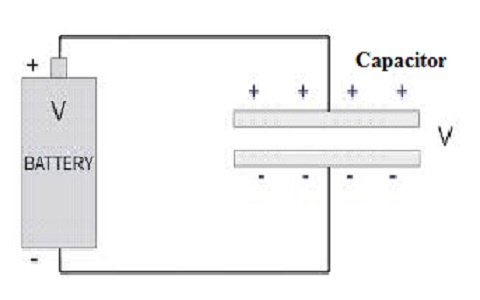
\includegraphics{images/Energy-Stored-in-Capacitor.jpg}
\end{figure}
The symbol for capacitors is shown in fig. \ref{fig:capa}
\begin{figure}
    \center 
    \caption{Capacitor symbol}
    \label{fig:capa}
    \begin{circuitikz}
        \draw (0,0) to[C] (0,1);
    \end{circuitikz}
\end{figure}
Capacitors, as many ECE students are aware, are immensely useful elements.
They can be used to store energy, stabilize signals, and detonators for explosives. 
If you imagine hooking up an uncharged capacitor to a battery, the voltage 
will look like fig. \ref{fig:capcharge}.
\begin{figure}
    \center 
    \caption{Capacitor charging}
    \label{fig:capcharge}
    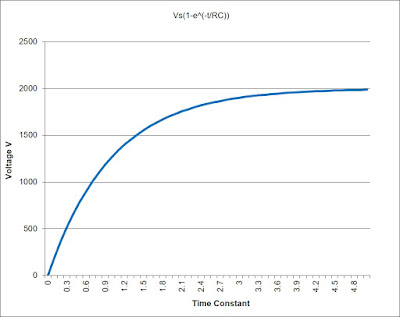
\includegraphics{images/2021-06-fig2.jpg}
\end{figure}
As more and more charge piles up on the plates of the capcitor, the incoming charge is 
gradually reduced until current flow essentially stops. Likewise, when discharging a capacitor, 
the current will initially be large as the charges piled up on the capacitor, but as charges 
on the plates flow around the wire and equalize, the current will gradually slow and eventually stop. 
The graph of voltage across a capacitor as it discharges looks like fig. \ref{fig:capdis}.
\begin{figure}
    \center 
    \caption{Capacitor discharging}
    \label{fig:capdis}
    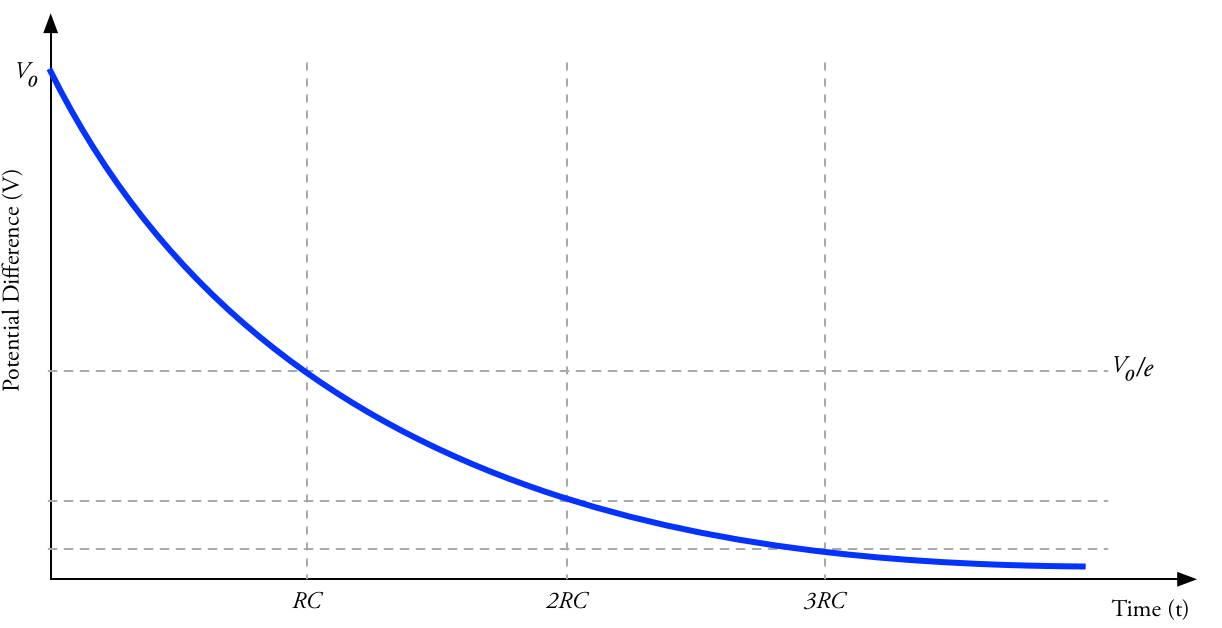
\includegraphics{images/Capacitor-discharge-curve.png}
\end{figure}
The relationship between the amount of charge piled up 
on a plate of the capacitor and the voltage of the capacitor is 
\[Q = C|V|,\]
where $C$ is known as the capacitance and is a constant specific to 
a certain capacitor. 
The capacitance is found via the formula 
\[C = \frac{\epsilon_0 A}{s},\]
where $A$ is the area of a plate and $s$ is the distance between plates. 
If capacitors are connected in parallel, you can imagine them as just one 
big capacitor with an area that is the sum of the individual areas and 
charge that is the sum of the charges. Thus the capacitance of parallel
capacitors is simply the sum of the individual capacitances, or mathematically, 
\[C_{total} = C_1 + C_2 + ... C_n = \sum_{i=1}^{n} C_i.\]
If we instead have capacitors in series, i.e. hooked up one after the other, 
we know that the voltage drop across the total will be equal to 
the sum of voltage drops across each capacitor. That is, 
\begin{align*}
    V_{total} &= V_1 + V_2 + \dots V_n \\
    \frac{Q}{C_{total}} &= \frac{Q}{C_1} + \frac{Q}{C_2} + \dots + \frac{Q}{C_n} \\
    \frac{1}{C_{total}} &= \frac{1}{C_1} + \frac{1}{C_2} + \dots + \frac{1}{C_n}
\end{align*}
\marginnote{
As I was typing these notes, my friend asked an excellent question about 
Kirchhoff's current law and capacitors. Since charge in piling up on 
the surfaces of the capacitor, the current never has a chance to flow across 
the capacitor and Kirchhoff's current law is violated. Kirchhoff's current law 
only holds for steady-state, and since the current is always changing across 
a capacitor, then we can't use Kirchhoff's current law! However, any negative charge 
that accumulates on one plate will push away charge on the other plate, so current 
entering one plate of a capacitor equals current leaving the other plate. 
}
In these cases we have been assuming a vacuum between the plates of the capacitor. 
If instead there is some insulating medium, the eletric field within 
the plates of the capacitor will be 
\[E = \frac{Q}{KA\epsilon_0}.\]
That implies 
\[C = K\frac{\epsilon_0 A}{s},\]
which tells us that the higher $K$ (the dieletric constant) is 
between the plates of a capacitor, the higher the capacitance. 
Manufacturers use this fact in making capacitors by putting
a highly insulating material between the plates, which are then rolled together
into a cylinder like in fig. \ref{fig:realcap}
\begin{figure}
    \center 
    \caption{Real capacitor}
    \label{fig:realcap}
    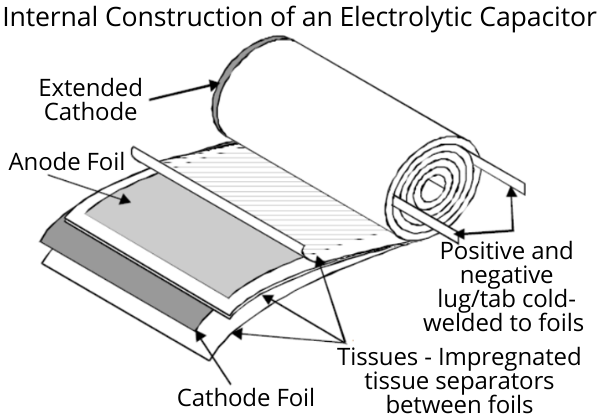
\includegraphics{images/internal-construction-(1).png}
\end{figure}

We can define the current 
density $\vec{J}$ as 
\begin{align*}
    \vec{J} &= \vec{J} = \frac{\vec{I}}{A}\\
    &= \frac{A|q|nu\vec{E}}{A} \\
    &= |q|nu\vec{E} \\
    &= \sigma \vec{E}
\end{align*}
where $\sigma$ is known as 
the conductivity and is 
intrinsic to the material. 
We can show that the equation 
$\vec{J} = \sigma \vec{E}$ is 
equivalent to Ohm's law $\Delta V = IR$. 
In a resistor of length $L$, 
\begin{align*}
    \Delta V &= - \int \vec{E} \cdot d\vec{L} \\
    &= EL
\end{align*}
So the current through the wire is 
\begin{align*}
    I &= \frac{\sigma AEL}{L}  \\
    &= \frac{\sigma A}{L}\Delta V\\
    &\rightarrow V = I \frac{L}{\sigma A} \\
    &= IR
\end{align*}
\marginnote{
Interesting fact, 
if the conductivity remains constant regardless
of how much current flows, then we call the material "ohmic". 
Resistors are pretty ohmic, while 
capacitors are not.}
There are several useful facts that 
arise out of this relationship. 
We can see that for 
a resistor,  $R = \frac{L}{\sigma L}$. 
Since the current through the resistor is 
$I = \frac{V}{R}$, increasing the 
length of the resistor decreases the 
current proportionally, while doubling the 
corss-sectional area of the resistor 
halves the resistance. This will be useful 
for both exams and homework. 

Now, let's turn our attention to 
circuits with a resistor and capacitor 
in series, as shown in fig. \ref{fig:RC}. 
\begin{figure}
    \caption{RC circuit}
    \label{fig:RC}
    \begin{circuitikz}
        \draw (0,0) to[V, l=$V_{emf}$, invert] (0,3)
        to[short, i=$I(t)$] (3,3)
        to[C, l=$Q(t)$] (3,1.5)
        to[R, l=$R$] (3,0)
        to[short] (0,0)
        ;
    \end{circuitikz}
\end{figure}
Such a circuit is known as an \emph{RC circuit}, for 
the resistor and capacitor within it. Let's recall 
that, for capacitors, $Q = CV$. It's also useful 
to remember the definition of current, $I = \frac{dQ}{dt}$. 
Let's now apply Kirchhoff's loop rule to the circuit as a whole. 
\begin{align*}
    V_{emf} &= V_C + IR \\
    &= \frac{Q}{C} + IR \\
    &= \frac{Q}{C} + \frac{dQ}{dt}R
\end{align*}
This is a first order differential equation. We can 
find the solution by assuming $Q(t) = ae^{bt}$. 
Solving the differential equation yields 
\[Q(t) = V_{emf} C (1-e^{-t/RC}).\]
If we wish to have the current, we can simply 
take the derivative of the above and find that 
\[I(t) = \frac{V_{emf}}{R}e^{-t/RC}.\]
\marginnote{
For some reason, physicists find it necessary to define 
the time constant $\tau = RC$. This unremarkable 
variable makes up a disproportionate quantity 
of exam questions, so it is worth your time to study it 
if you care about grades. 
}
Let's now consider a discharging RC circuit. After the capcitor 
has stored up all the voltage, we disconnect the battery and let 
the capacitor spill out its charge. The circuit diagram in this case looks 
like fig \ref{fig:RCdischarge}. 
\begin{figure}
    \caption{Discharging RC circuit}
    \label{fig:RCdischarge}
    \begin{circuitikz}
        \draw (0,0) to[short] (0,3)
        to[R, l=$R$] (3,3)
        to[C, l=$Q(t)$] (3,1.5)
        to[short] (3,0)
        (0,0) to[short, i=$I(t)$] (3,0)
        ;
    \end{circuitikz}
\end{figure}
In this case, Kirchhoff's loop rule yields
\begin{align*}
    0 &= I(t)R - \frac{Q(t)}{C} \\
    &= \frac{dQ(t)}{dt} - \frac{Q(t)}{C}
\end{align*}
The solution of which is 
\[Q(t) = V_{emf} C e^{-t/RC}.\]
Again, differentiating yields 
\[I(t) = \frac{V_{emf}}{R} e^{-t/RC}.\]

Now, let's examine how to find the equivalent
resistance of resistors in series and parallel.
First, let's define each of these terms. 
\begin{itemize}
    \item[Series] One after the other. 
    \item[Parallel] Share two nodes, i.e. next to each other. 
\end{itemize} 
If resistors are in series, the current 
through each is the same. If they are in 
parallel, the voltage across each is the same. 
Here is how we find the combined resistance if 
resistors $R_1, R_2, \dots R_n$ are in series: 
\[R_{eq} = R_1 + R_2 + \dots R_N.\]
If they are in parallel, the equivalent 
resistance is given by 
\[\frac{1}{R_{eq}} = \frac{1}{R_1} + \frac{1}{R_2} + \dots + \frac{1}{R_n}.\]

If we have a circuit with $N$ nodes and $B$ branches, 
then the number of independent nodes is $N-1$ and 
the number of independent loops is $B-N+1$. 
In fig. \ref{fig:numn} there are two nodes (intersections of wires)
and three branches (wires between two nodes). 
\begin{figure}
    \center 
    \caption{Nodes and branches}
    \label{fig:numn}
    \begin{circuitikz}
        \draw (0,0) to[short, i=$I_1$] (0,3)
        to[R, l=$R_1$] (3,3)
        to[R, i = $I_2$, l = $R_2$] (3,0)
        to[V, l=$V_1$] (0,0)
        ;
        \draw (3,0) to[short] (6,0)
        to[short, i=$I_3$] (6,3)
        to[R, l=$R_3$] (3,3)
        ;
    \end{circuitikz}
\end{figure}
Ergo, we will have $2-1 = 1$ independent nodes 
and $3-2+1 = 2$ independent loops. 
This will give us a total of $1 + 2$ equations, 
which will be enough to solve our circuit 
(i.e. find all currents). These equations are 
\begin{align*}
    I_2 &= I_1 + I_3 \\
    5 V - I_1 R_1 - I_2 R_2 &= 0 \\
    I_2 R_2 - I_3 R_3 &= 0
\end{align*}
\marginnote{It is useful to know how 
to solve systems of linear equations with 
linear algebra.}

Let's now consider capacitors in series and 
parallel. For capacitors in parallel, 
the equivalent capacitance is simply the sum 
of the individual capacitances: 
\[C_{eq} = C_1 + C_2 + \dots + C_n.\]
If they are in series instead, 
\[\frac{1}{C_{eq}} =frac{1}{C_1} + \frac{1}{C_2} + \dots + \frac{1}{C_n}.\]

A term that often arises when discussing circuits is \emph{power}. 
Power is defined as $P = I \Delta V$. For 
resistors, $P = I \Delta V = I \times IR = I^2 R = \frac{V^2}{R}$. 
That means that if you have lightbulbs in series 
(so their current is the same). Then the 
one that dissipates the most power 
(and is therefore the brightest) will 
be the one with the greatest resistance. 
If you have lightbulbs in parallel and a voltage source $V$, 
then the power dissipated by each will be 
\begin{align*}
    P_1 &= \frac{V^2}{R_1} \\
    P_2 &= \frac{V^2}{R_2} \\
    \dots \\\
    P_n &= \frac{V}{R_n}.
\end{align*}
This means that the one with the smallest 
resistance will dissipate the most power. 

Let's now consider \emph{ammeters}, 
\emph{voltmeters}, and \emph{ohmmeters}. 
\begin{itemize}
    \item[Ammeter] measures current (Amps)
    \item[Voltmeter] measures voltage difference (Volts)
    \item[Ohmmeter] measures resistance (Ohms)  
\end{itemize}
An ammeter is inserted into a circuit in series with the circuit
element whose current you want to measure. It has a low resistance 
so it doesn't impede the current. A voltmeter is connected 
in parallel with the element. It has a very high 
internal resistance so it doesn't affect the current much 
(it still needs to take some current, since it 
works by measuring the voltage drop across 
the internal resistor). An ohmemter is connected 
in series and contains a small voltage source. 
It calculates the resistance by taking the 
value of the voltage and dividing it by 
the current observed in the contained ammeter. 
\marginnote{All of these are ideal components, 
but in reality, ammeters have internal resistance just 
as batteries and wires do.}

\section{Magnetic force}
The force $F$ on a charge $q$ moving with velocity
$\vec{v}$ through a region of space with electric field $\vec{E}$
and magnetic field $B$ is given by
\[\vec{F} = q\vec{E} + q\vec{v}\times\vec{B}.\]
We can isolate the magnetic term and find that the 
force of a magentic field on a moving charge is 
\begin{align*}
    \vec{F}_B &= q\vec{V} \times \vec{B} \\
    |vec{F}_B| &= |q||\vec{V}||\vec{B}|\sin(\theta)
\end{align*}
Computing the cross product is tedious, so here's a \emph{handy} 
shortcut to determining direction. 
If you point your pointer finger in 
the direction the positive charge is moving, and then your 
middle finger in the direction of the magnetic field, your 
thumb points in the direction of the magnetic force pushing 
on the moving charge. This is known as the \emph{right hand rule}. 
The right hand rule immediately gives you the direction if 
the charge in question is positive. If the charge is negative, the direction 
is opposite to the direction given by the right hand rule.
\begin{figure}
    \center 
    \caption{Right hand rule}
    \label{fig:rhr}
    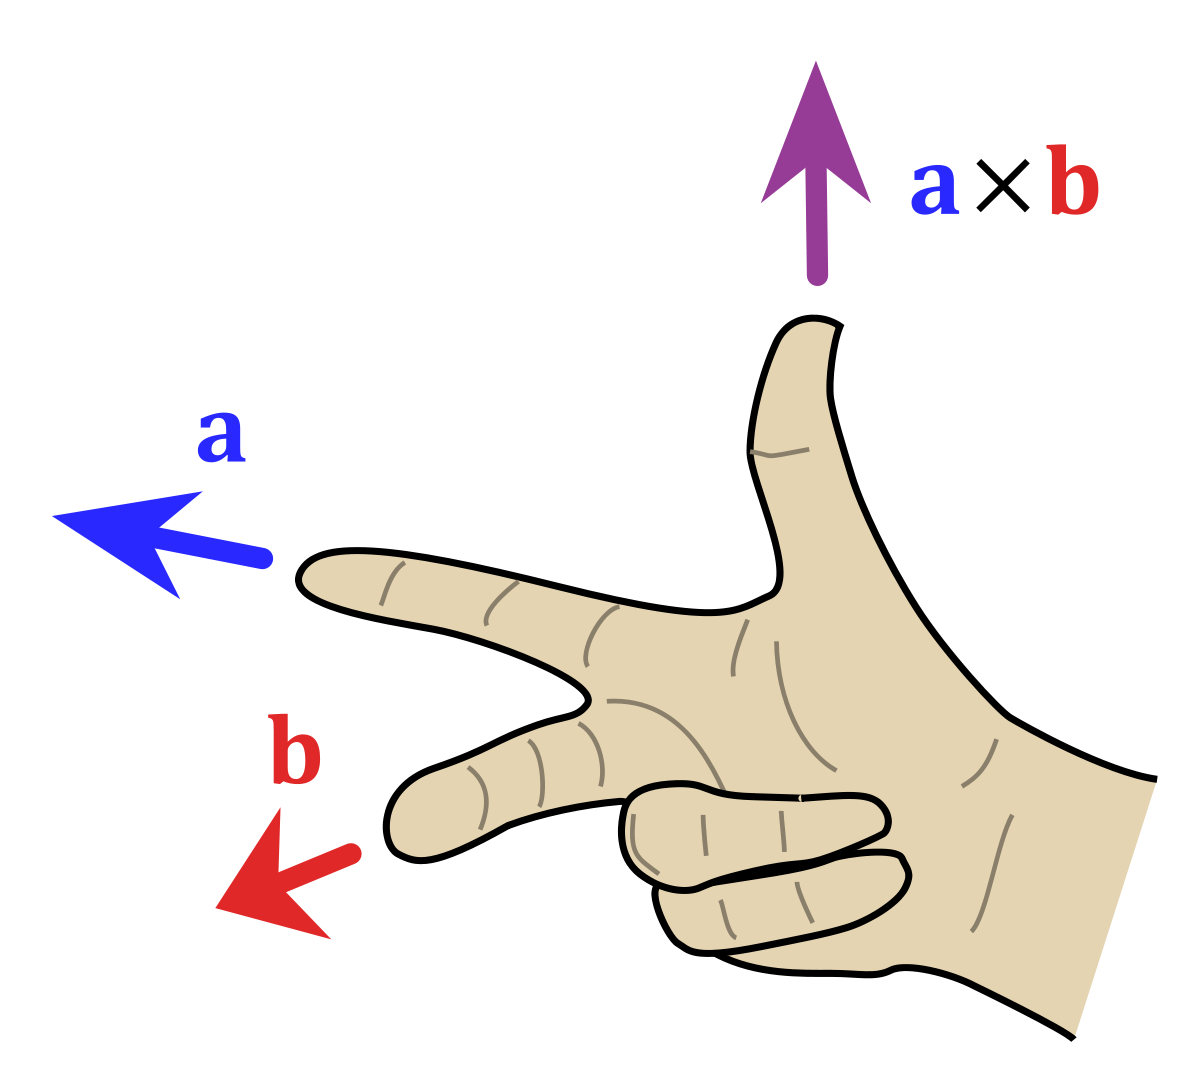
\includegraphics{images/1200px-Right_hand_rule_cross_product.svg.png}
\end{figure}
The magnetic force on a charged object that moves in a
magnetic field does not do any work, because it's
perpendicular to $\vec{v}$.
Therefore the magnetic force cannot change the magnitude of the
velocity of a charged object, but can change the direction
of motion. 
\marginnote{The magentic force is always perpindicular to velocity,
and can only change the direction, not the magnitude. Sound familiar?
This is what centrifugal force does. Indeed, magnetism causes a charge to 
move in a circle if there is a constant magnetic field perpindicular to the velocity.}
We can find the momentum of a moving particle in a magnetic field, which actually turns 
out to be quite useful. If the particle moves in a circle of radius $R$, then 
\begin{align*}
    \vec{r} &= R\hat{r} \\
    \vec{v} &= R\omega\hat{\theta} \\
    \vec{p} &= \gamma m \vec{v}, \text{ where } \gamma = \frac{1}{\sqrt{1-\frac{v^2}{c^2}}} \\
    \frac{d\vec{p}}{dt} &= -\gamma mR\omega^2\hat{r} \\
    |\frac{d\vec{p}}{dt}| &= \gamma mR\omega^2 \\
    &= p\omega \\
    &= |q|vB \\
    p &= |q|BR
\end{align*}
\marginnote{The Lorentz factor $\gamma$ is here 
to ensure our equation for momentum is still 
valid for relativistic speeds. If the speeds 
are much lower than the speed of light ,
$\gamma \approx 1$.}
This is very useful for particle physicists, 
since they can measure the strength of the 
eletric field and the radius of the circle. 
Cyclotrons, a type of particle accelerator, 
take advantage of this behavior. Our equation for 
momentum naturally leads to some useful 
expressions for cyclotrons. 
\begin{align*}
    \omega &= \frac{|q|B}{m} \\
    f &= \frac{|q|B}{2\pi m} \\
    T &= 2\pi \frac{m}{|q|B}
\end{align*}
We can inject different particles into 
a cyclotron, observe their frequency, and 
draw conclusions about their mass. 
This allows us to do things such as 
determine isotopes, identify fundamental 
particles, and impress the Nobel prize committee. 
Chemists actually often need to seperate ions 
by mass and measure the mass of each type of ion, 
so we've made a specific instrument for them called 
a \emph{mass spectrometer} (fig. \ref{fig:massspec}). 
\begin{figure}
    \center 
    \caption{Mass spectrometer} 
    \label{fig:massspec}
    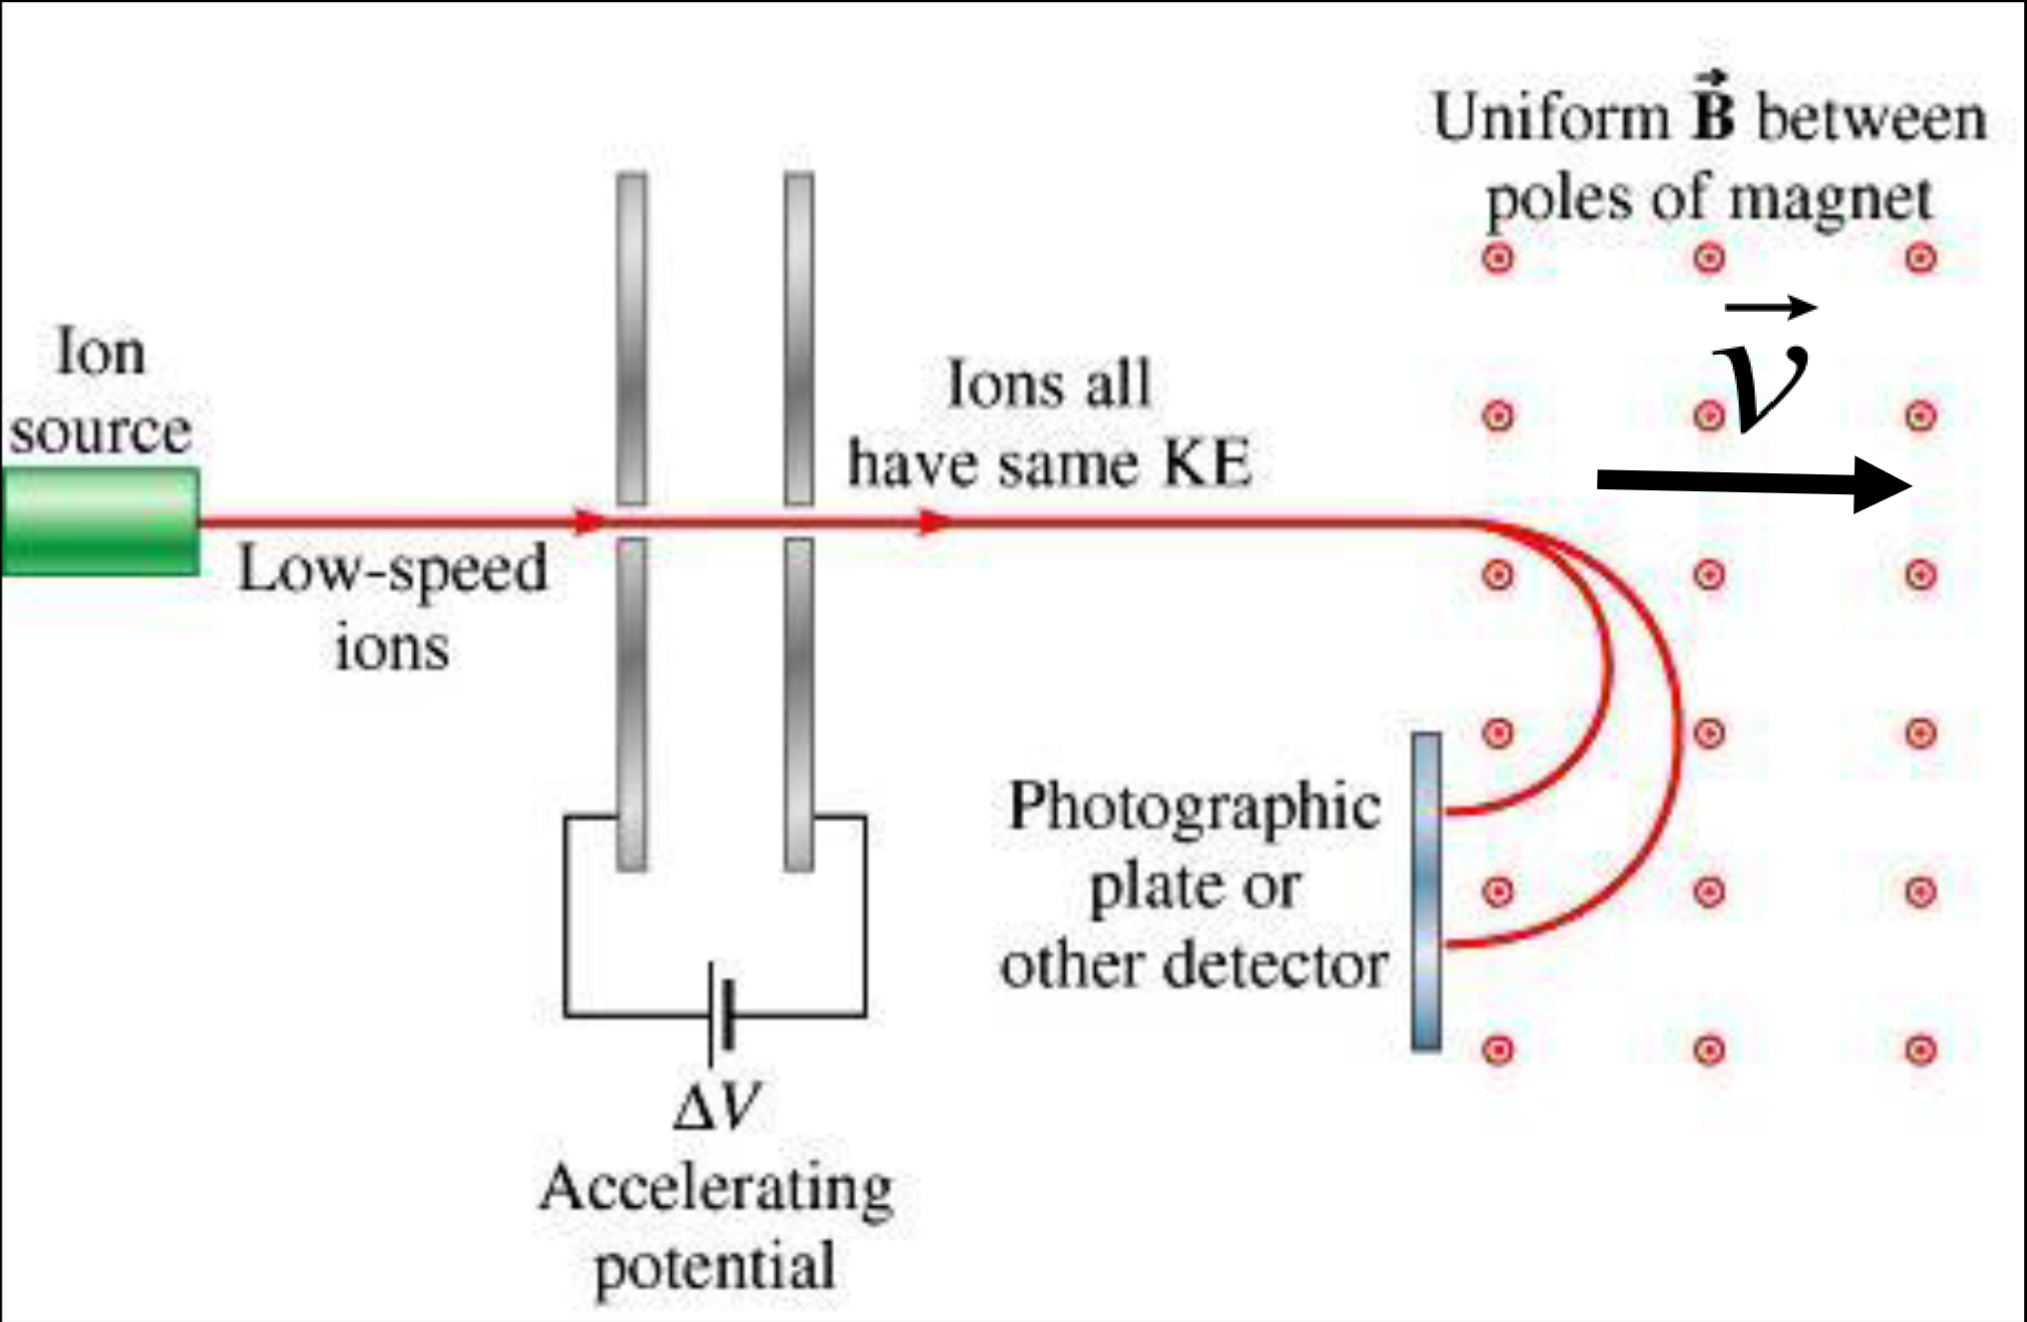
\includegraphics{images/massspec.png}
\end{figure}
We can do a little bit of work and find 
that 
\[\frac{m}{q} = \frac{B^2 R^2}{2|\Delta V|}.\]

Recall the Biot-Savart law, which states 
that for a current-carrying wire 
\[\vec{B} = \frac{\mu_0}{4\pi} \frac{I \Delta \vec{l} \times \hat{r}}{|r|^2}.\]
Since this wire creates a magnetic field, 
it will exert a force on other wires. 
If these wires have current $I_1$, $I_2$ and are 
seperated by a distance $d$, this force 
is given by 
\[F = \frac{\mu_0}{4\pi} \frac{2I_1 I_2}{d} \Delta l.\]
\marginnote{If you have a wire twisted into a non-circular shape and run current through it, 
the reflexive magnetic force will expand the wire into a circle.}

We can use the fact that a magnetic field exerts a force 
on a wire with current to create machines that turn electrical energy into 
physical energy. Consider fig. \ref{fig:magtorque}. 
\begin{figure}
    \center 
    \caption{Torque}
    \label{fig:magtorque}
    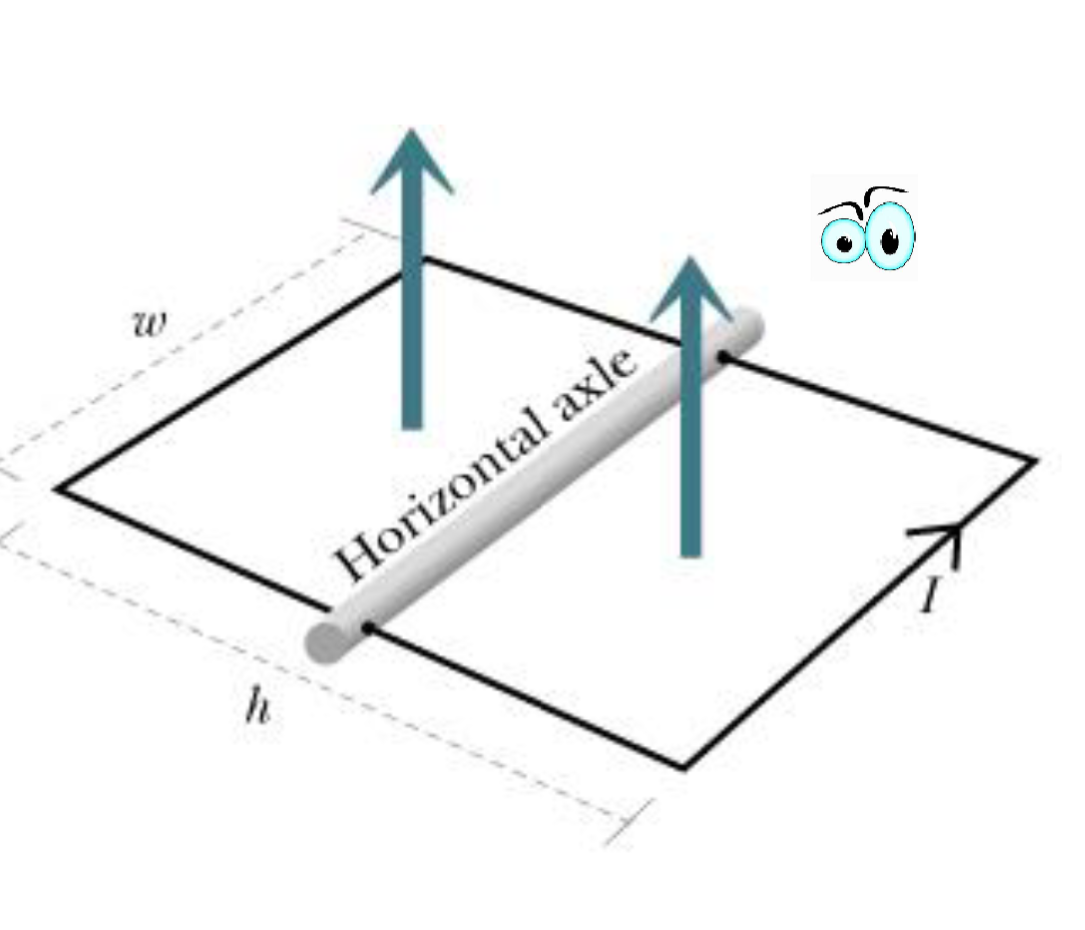
\includegraphics{images/Screenshot 2023-11-06 100829.png}
\end{figure}
In this example, 
\begin{align*}
    \vec{F} &= I\Delta \vec{l} \times \vec{B} \\
    |F| &= IwB \\
    |F_{\perp}| &= IwB\sin(\theta) \\
    \mu &= IA \\
    &= Iwh \\
    \tau &= IwhB\sin(\theta) \\
    &= \mu B \sin(\theta) \\
    &= \vec{\mu} \times \vec{B}
\end{align*}
This equation, $\vec{\mu} \times \vec{B}$, is valid for a loop of any shape. 

We may also go in the opposite direction. By rotating a loop in a magnetic field, 
we may convert mechanical energy to electrical energy. Working through the math, 
we will find that 
\[emf(t) = A\omega B \sin(\omega t,\]
where $\omega$ is the rotational speed, $A$ is the area, and $B$ is the strength of 
the magnetic field. At any time during the rotation, the loop has potential given by 
\[U_m = =-\vec{\mu} \cdot \vec{B},\]
which is true for a general magnetic dipole. The force on a magnetic dipole 
is 
\begin{align*}
    F_x &= \mu \frac{dB_x}{dx} \\
    &= -\frac{\mu_0}{4 \pi} \frac{6 \mu_1 \mu_2}{x^4} \text{ (in the case of two dipoles)}
\end{align*}

Consider a moving bar in an applied magnetic field. The work done on the bar 
is $ W= ILB \Delta x$. Moving the bar through the field exerts a force on 
the electrons within the bar, causing a current to flow throughout the bar. 
If the bar has a wire hooked up, the current can flow through the wire and be 
used to deliver power to a load. If there is no wire, charge will just pile 
up at each end. 

\section{Hall Effect}
\defn{Hall effect}{The Hall effect is the production of a potential 
difference (the Hall voltage) across an electrical conductor that 
is transverse to an electric current in the conductor and to an 
applied magnetic field perpendicular to the current}. 
\begin{figure}
    \center 
    \caption{Hall effect}
    \label{fig:hall}
    \includegraphics*{images/Hall_Effect_Measurement_Setup_for_Electrons.png}
\end{figure}
Since moving charges in a magnetic field experience a force perpindicular to their 
direction of motion, positive charges will be forced to one side of the material and 
negative charges to the other. This creates a potential difference across the material, 
called the Hall voltage. In steady-state, the force of these accumulated charges 
will exactly cancel the magnetic force. 
By measuring current, voltage across the material in the direction of current, 
and voltage across the transverse, you can figure out if the charge carriers 
in a material are positive or negative. 
The steps to do so are easy: 
\begin{enumerate}
    \item Apply a magentic field.
    \item Apply a current across the material. 
    \item Measure the Hall voltage. 
\end{enumerate}

\section{Special Relativity}
Special relativity is based on two
postulates:
\begin{itemize}
    \item Laws of physics are invariant in all
    inertial frames of reference (with constant $v$).
    \item The speed of light in the vacuum is the same
    for all observers.
\end{itemize}

Special relativity predicts how magnetic and eletric 
fields transform when you change from one inertial frame of 
reference to another.

Imagine you have a current $I$ flowing in a wire, and an electron 
travelling next to it. From the viewpoint of a stationary observer, 
we would observe that the electron moves down due to the force from 
the wire. However, imagine you are travelling with the electron. Then 
its velocity relative to you is zero, and so the force it experiences is 
zero. How can we resolve this conundrum? The answer is with relativity. 
In classical physics, we would desribe this system as 
\marginnote{The apostrophe "'" indicates that we are transforming from 
one frame of reference to another.}
\begin{align*}
    t' &= t \\
    x' &= x - vt \\
    y' &= y \\
    z' &= z
\end{align*}
In relativity, a corrective factor arises and we have that
\begin{align*}
    \gamma &= \frac{1}{\sqrt{1 - \frac{v^2}{c^2}}} \\
    t' &= \gamma \left(t - \frac{vx}{c^2}\right) \\
    x' &= \gamma (x - vt) \\
    y' &= y \\
    z' &= z
\end{align*}
What we find is that the electron still experiences a force, 
but now, there is an eletric field from the wire, and this is 
what repels the electron. We can find expressions for the electric 
and magnetic fields incorporating relativity as well. 

Space and time warp to keep the speed of light constant 
for all observers! Namely, 
\begin{align}
    L_{obs} &= \frac{L}{\gamma} \\
    t_{obs} &= \gamma \times t 
\end{align}
It is possible to deduce the Boit-Savart law from special 
relativity alone! Consider a frame where a charged particle is still. 
The eletric field is given by 
\[\vec{E} = \frac{1}{4 \pi \epsilon_0} \frac{q}{r^2} \hat{r},\]
while the magentic field $B$ is zero. Say you have another frame, 
the \emph{primed} frame, what is moving to the right with speed $v$. 
Then we observe that 
\[B_z' = \gamma (B_z - \frac{v E_y}{c^2}).\]
Substituting in and assuming $v << c$, we find that 
\[B_z' =  -\frac{\mu_0}{4 \pi} \frac{qv}{r^2}.\]
So we find that the magnetic force is just the electric force under 
a relativistic transformation! That hints at a relation between the mangetnic 
and eletric fields, which we shall soon see are intertwined. 

\section{Gauss's Law}
To get into Gauss's law, it will first be useful to understand \emph{flux}. 
\defn{Flux}{a measure of the number of electric or magnetic field lines 
passing through a surface.} 
It may be useful to imagine flux as the flow of water through an area. 
Just as with water flowing, there must be a source. In the case of electric field 
the source is a charge. Suppose you have water flowing through a loop of area $A$. 
The flux is the volume of water per time, so we have that 
\begin{align*}
    \phi &= \frac{V}{\Delta t} \\
    &= \frac{v \Delta t A}{\Delta t} \\
    &= vA
\end{align*}
However, the amount of water flowing through depends on the angle between the 
velocity and the loop. If the loop just cuts the water in half (if it is perpindicular)
then there is no water flow through the loop. The effective area in that case becomes 
$A \cos(\theta)$, and our equation becomes 
\[\phi = vA\cos(\theta).\]
In the case of the electric field, the flux is defined as
\begin{align*}
    \phi &= \sum (\vec{E} \cdot \hat{n}) dA \\
    &= \sum E\cos(\theta) dA \\
    &= \int \vec{E} \cdot d\vec{A} \\
    &= \oint \vec{E} \cdot d\vec{A}
\end{align*}
\marginnote{Don't let the symbol 
$\oint$ scare you. It simply means 
that this is an integral on a 
closed surface, such as a sphere, a cube, etc.
We will usually not even need to compute 
the integral if we can exploit the symmetry 
of a problem.}
Now, here is Gauss's law: 
If you have a charge $Q$ enclosed in a surface $S$, 
then 
\begin{align*}
    \phi &= \oint_S \vec{E} \cdot d\vec{A} \\
    &= \frac{Q}{\epsilon_0}
\end{align*}
Not so bad! To get a little intuition, consider
the case where you have a closed surface with 
no charge within, but the surface is still in an
electric field. Then any eletric field lines that 
flow in must pass out again, so the net flux is 
zero, just as $\frac{0}{\epsilon_0}$ is zero!
Note that the law works for any closed surface, so 
the flux through a sphere, cube, cylinder, etc. 
will all be the same if the same charge in enclosed. 
The size doesn't matter, either!

There exists a comparable law for the magnetic field, stating
\[\oint_S \vec{B} \cdot d \vec{A} = 0.\]

\end{document}
